\section{Mass generation at one scale implies the cube condition}\label{sec:massgen}

Theorem~\ref{thm:B} reduces the continuum gap to statement (D), a cube
condition uniform along the tuning. This section reduces (D) in turn to a
hypothesis of a different kind, closer to the physics: a uniform decay of
correlations between the gauge-invariant observables of two slabs of a box
separated by a slab of physical width about $\ell/2$, for every boundary
condition. If the maximal correlation is at most $c<\frac12$, then the cube
condition holds with $\varpi=(1-2c)^4/32$ (Theorem~\ref{thm:D}). The value
$\frac12$ is the exact limit of the method (Proposition~\ref{prop:gausschain}
in Appendix~\ref{app:obstructions}); the hypothesis implies exponential decay
of gauge-invariant correlations under every boundary condition
(Proposition~\ref{prop:alldecay}); and it holds in two dimensions along the
weak-coupling tuning (Theorem~\ref{thm:twod}). In four dimensions it is a
form of mass generation at the physical scale and it is not proved here.

\subsection{Boxes, boundary conditions and gauge-invariant observables}

In this section $G\subset\U(N)$ is compact and nontrivial, $\varphi$ is a
positive continuous class function on $G$, $\lambda$ denotes normalised Haar
measure on $G$ or on a product of copies of $G$, and
$\omega_\varphi=\log(\max\varphi/\min\varphi)$. Links of $\Z^4$ are written
$(y,\nu)$ with base point $y$, from $y$ to $y+e_\nu$. A \emph{box} is a set
$Q=\prod_{i=1}^4[\alpha_i,\alpha_i+s_i)\cap\Z$ with integers $s_i\ge1$, its
\emph{widths}, and $V(Q)$ is the set of links with base point in $Q$. For an
exterior configuration $\omega\in G^{E(\Z^4)\setminus V(Q)}$ let
$\nu^\omega_Q$ be the probability measure on $G^{V(Q)}$ with density
proportional to $\prod_{p\cap V(Q)\ne\emptyset}\varphi((\sigma,\omega)_p)$
with respect to $\lambda$, a finite product. It is the conditional law of
$U_{V(Q)}$ given the other links under any Gibbs measure with weight
$\varphi$, and on a torus $\Lambda_L$ with all $s_i\le L-3$ it is the
conditional law of the torus measure.\footnote{The plaquettes meeting $V(Q)$
have their links based in $\prod_i[\alpha_i-1,\alpha_i+s_i]$, which embeds in
$\Lambda_L$ when $s_i\le L-3$.} For $A\subset V(Q)$ write $E_A$ for the
conditional expectation under $\nu^\omega_Q$ given $\sigma_{V(Q)\setminus A}$;
its regular version is integration against the measure on $G^A$ with density
proportional to $\prod_{p\cap A\ne\emptyset}\varphi(U_p)$, which is jointly
continuous in all variables. In particular, if $Q'\subset Q$ is a box, the
conditional law of $\sigma_{V(Q')}$ under $\nu^\omega_Q$ given
$\sigma_{V(Q)\setminus V(Q')}=\eta$ is $\nu^{(\eta,\omega)}_{Q'}$.

A vertex $v$ is \emph{interior} to $Q$ if the eight links incident to $v$ lie
in $V(Q)$. Let $\mathcal G_Q$ be the group of $h\in G^{\Z^4}$ with $h_v=1$ at
every vertex not interior to $Q$, acting by $(h\sigma)_{(y,\nu)}=h_y
\sigma_{(y,\nu)}h_{y+e_\nu}^{-1}$; it fixes every link outside $V(Q)$, whose
end points are not interior. Let $\mathcal A^\omega_Q$ be the set of real
$F\in L^2(\nu^\omega_Q)$ with $F\circ h=F$ almost surely for every $h\in
\mathcal G_Q$: the gauge-invariant observables of the box, the boundary
condition having fixed the gauge on the boundary.

\begin{lemma}\label{lem:boxinv}
Let $Q$ be a box, $\omega$ an exterior configuration and $\nu=\nu^\omega_Q$.
\begin{enumerate}[label=\textup{(\roman*)},leftmargin=*]
\item $\nu$ is invariant under $\mathcal G_Q$.
\item For every $S\subset V(Q)$, each $h\in\mathcal G_Q$ maps
$\sigma(\sigma_S)$ onto itself, and $E_A(F\circ h)=(E_AF)\circ h$ for
$A\subset V(Q)$ and $F\in L^2(\nu)$.
\item $\mathcal A^\omega_Q$ is a closed subspace that contains the constants
and is preserved by every $E_A$. Every $F\in\mathcal A^\omega_Q$ has a
version $\tilde F$ with $\tilde F(h\sigma)=\tilde F(\sigma)$ for all $h$ and
$\sigma$, and if $F$ is $\sigma(\sigma_S)$-measurable, $\tilde F$ can be taken
$\sigma(\sigma_S)$-measurable.
\end{enumerate}
\end{lemma}

\begin{proof}
(i) $h$ multiplies each link on the left and on the right by fixed elements,
so it preserves $\lambda$. Since $h$ fixes the links outside $V(Q)$,
$(h\sigma,\omega)=h\cdot(\sigma,\omega)$, and the holonomy of a plaquette
with base point $y$ is conjugated by $h_y$; $\varphi$ is a class function,
so the density is invariant.

(ii) $(h\sigma)_e$ is a function of $\sigma_e$ alone and $h^{-1}\in\mathcal
G_Q$, so $h$ maps $\sigma(\sigma_S)$ onto itself. For a bounded
$\sigma(\sigma_{V(Q)\setminus A})$-measurable $K$, by (i),
$\nu((F\circ h)K)=\nu(F\,(K\circ h^{-1}))=\nu((E_AF)(K\circ h^{-1}))=
\nu(((E_AF)\circ h)K)$, and $(E_AF)\circ h$ is
$\sigma(\sigma_{V(Q)\setminus A})$-measurable.

(iii) By (i) each map $F\mapsto F\circ h$ is unitary, so its fixed space is
closed, and so is the intersection of these spaces; (ii) gives the
invariance under $E_A$. The group $\mathcal G_Q\cong G^I$, $I$ the finite set
of interior vertices, is compact and acts continuously. For a measurable
version $F_0$ put $\tilde F(\sigma)=\int F_0(h\sigma)\,dh$ where
$\int|F_0(h\sigma)|\,dh<\infty$, and $\tilde F(\sigma)=0$ elsewhere. By the
invariance of Haar measure under right translations, the set where the
integral converges and $\tilde F$ are invariant under every $k\in\mathcal
G_Q$. For each $h$, $F_0(h\sigma)=F_0(\sigma)$ for almost every $\sigma$, so
by Fubini's theorem, for almost every $\sigma$ the equality holds for almost
every $h$, and $\tilde F=F_0$ almost surely. If $F_0$ is a function of
$\sigma_S$, so is $\sigma\mapsto F_0(h\sigma)$ for each $h$, and so is
$\tilde F$.
\end{proof}

\begin{definition}\label{def:rho}
Let $Q$ be a box, $i$ a coordinate, and $Q=Q_-\cup Q_0\cup Q_+$ a splitting
into three nonempty boxes, consecutive in the coordinate $i$ in this order:
the \emph{outer parts} $Q_\pm$ and the \emph{middle} $Q_0$. For an exterior
configuration $\omega$ put $\nu=\nu^\omega_Q$ and
\[
\rho^\omega(Q_-,Q_+)=\sup|\nu(XY)|,
\]
the supremum over $X\in\mathcal A^\omega_Q$ measurable with respect to
$\sigma_{V(Q_-)}$ and $Y\in\mathcal A^\omega_Q$ measurable with respect to
$\sigma_{V(Q_+)}$ with $\nu(X)=\nu(Y)=0$ and $\nu(X^2)=\nu(Y^2)=1$ (the
supremum of the empty set being $0$).
\end{definition}

This is the maximal correlation\footnote{The maximal correlation of two
random variables, the supremum of the correlations of square-integrable
functions of each, was introduced by Hirschfeld and by
Gebelein~\cite{Geb41}; for jointly Gaussian variables it equals the
absolute value of the ordinary correlation.} between the gauge-invariant
observables of the two outer parts, the middle being integrated out, under
the boundary condition $\omega$. By the Cauchy--Schwarz inequality
$\rho^\omega\le1$.

\begin{definition}\label{def:M}
Let $d\ge2$, $m\ge4$ and $w\ge1$ be integers and $0\le c\le1$.
\begin{enumerate}[label=\textup{(\roman*)},leftmargin=*]
\item $(\mathrm M_{d,m}(c))$: $\rho^\omega(Q_-,Q_+)\le c$ for every box $Q$
all of whose widths lie in $[2d-1,md-1]$, every coordinate $i$ in which $Q$
has width $3d-1$, the splitting in which $Q_-$, $Q_0$, $Q_+$ have widths
$d$, $d-1$, $d$ in the coordinate $i$, and every exterior configuration
$\omega$.
\item $(\mathrm M^*_w(c))$: $\rho^\omega(Q_-,Q_+)\le c$ for every box $Q$,
every coordinate $i$, every splitting whose middle has width $w$ in the
coordinate $i$, the outer parts being of any widths, and every $\omega$.
\end{enumerate}
\end{definition}

\begin{figure}[t]
\centering
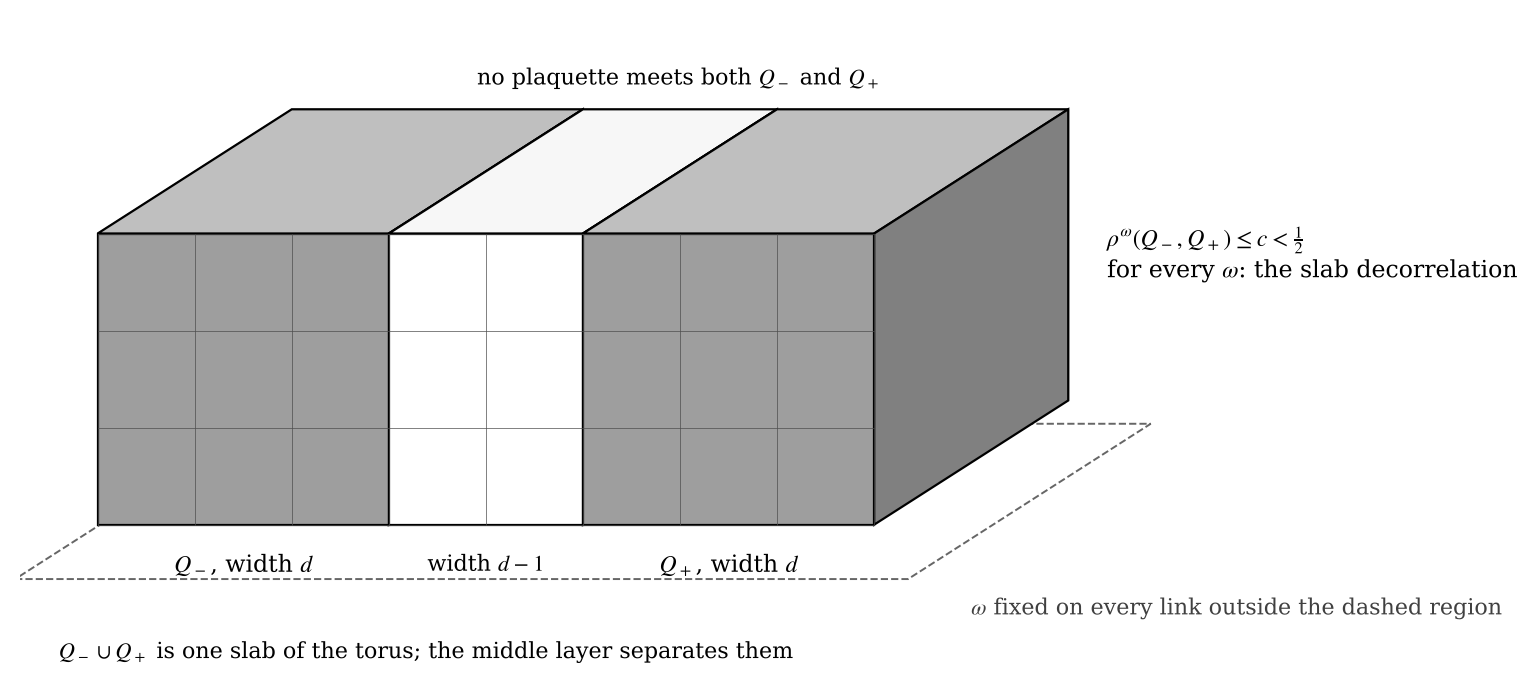
\includegraphics[width=\textwidth]{figures/fig_slab.png}
\caption{The splitting of Definition~\ref{def:M}: in the coordinate $i$ a box $Q$ of width $3d-1$ is cut into $Q_-$, $Q_0$, $Q_+$ of widths $d$, $d-1$, $d$; the middle is integrated out, the exterior configuration $\omega$ is fixed, and $\rho^\omega(Q_-,Q_+)$ is the maximal correlation of gauge-invariant observables of the two outer parts. No plaquette meets both $Q_-$ and $Q_+$, since the base points of the links of a plaquette differ by at most one in each coordinate and $d\ge2$.}
\label{fig:slab}
\end{figure}

The boxes of $(\mathrm M_{d,m}(c))$ are fat: all their widths are at least
$2d-1$. The restriction matters. In two dimensions the same condition for
boxes of width one in a transverse direction fails along the weak-coupling
tuning, through a broken global symmetry of a pinned strip, while the fat
form holds there (Theorem~\ref{thm:twod} and Proposition~\ref{prop:strip}
in Appendix~\ref{app:obstructions}). At $\varphi\equiv1$ the links are
independent under $\nu^\omega_Q$, so $\rho^\omega=0$ and both conditions hold
with $c=0$. Along the tuning, with $d\approx\ell/(2a)$, $(\mathrm
M_{d,m}(c))$ is a statement at the physical separation $(d-1)a\approx\ell/2$
in boxes of physical size at most about $m\ell/2$, uniform in the boundary
condition, and stated for all square-integrable gauge-invariant observables
of the two regions rather than for pairs of local ones.

\subsection{Two projections and a chain of projections}

\begin{lemma}\label{lem:friedrichs}
Let $P_1,P_2$ be orthogonal projections on a real Hilbert space $\mathcal K$,
$\mathcal N$ a closed subspace of $\operatorname{ran}P_1\cap
\operatorname{ran}P_2$, and suppose that $|\ip xy|\le c\|x\|\|y\|$ for all
$x\in\operatorname{ran}P_1\ominus\mathcal N$ and $y\in\operatorname{ran}P_2
\ominus\mathcal N$. Put $Q_k=I-P_k$ and $X=Q_1+Q_2$. Then $X^2\ge(1-c)X$,
that is, $Q_1Q_2+Q_2Q_1\ge-c(Q_1+Q_2)$.
\end{lemma}

\begin{proof}
For $n\in\mathcal N$, $P_kn=n$, so $Xn=0$; as $X$ is self-adjoint it also
preserves $\mathcal N^\perp$. Let $g\in\mathcal N^\perp$. Then $P_kg\perp
\mathcal N$, since $\ip{P_kg}n=\ip g{P_kn}=\ip gn=0$, so with $p=\|P_1g\|$
and $q=\|P_2g\|$, $|\ip{P_1g}{P_2g}|\le cpq$. Put $s=\ip g{(P_1+P_2)g}=
p^2+q^2$. Then $\|(P_1+P_2)g\|^2=p^2+q^2+2\ip{P_1g}{P_2g}\le(1+c)(p^2+q^2)$
and $s\le\|g\|\|(P_1+P_2)g\|\le\|g\|((1+c)s)^{1/2}$, so $s\le(1+c)\|g\|^2$
and $\ip g{Xg}=2\|g\|^2-s\ge(1-c)\|g\|^2$. So $X=0$ on $\mathcal N$, and on
$\mathcal N^\perp$ the operator $X-(1-c)$ is nonnegative and commutes with
$X\ge0$; hence $X^2-(1-c)X=X^{1/2}(X-(1-c))X^{1/2}\ge0$ there. Finally
$X^2-X=Q_1Q_2+Q_2Q_1$.
\end{proof}

The angle between $\operatorname{ran}P_1\ominus\mathcal N$ and
$\operatorname{ran}P_2\ominus\mathcal N$ is the Friedrichs angle of the two
ranges, and the lemma is a form of the classical relation between that angle
and the rate of the alternating projections~\cite{Deu01}.

\begin{lemma}\label{lem:chain}
Let $Q_0,\dots,Q_M$ be orthogonal projections on a real Hilbert space
$\mathcal K$ with $Q_tQ_{t'}=Q_{t'}Q_t$ whenever $|t-t'|\ge2$ and
$Q_tQ_{t+1}+Q_{t+1}Q_t\ge-c(Q_t+Q_{t+1})$ for $0\le t<M$, with $0\le c<
\frac12$. Then $H=\sum_tQ_t$ satisfies $H^2\ge(1-2c)H$, and $\ip g{Hg}\ge
(1-2c)\|g\|^2$ for every $g\perp\ker H$.
\end{lemma}

\begin{proof}
$H^2=\sum_tQ_t+\sum_{t<M}(Q_tQ_{t+1}+Q_{t+1}Q_t)+\sum Q_tQ_{t'}$, the last
sum over the ordered pairs with $|t-t'|\ge2$. Each such $Q_tQ_{t'}$ is a
product of commuting projections, hence a projection and nonnegative. The
middle sum is at least $-c\sum_{t<M}(Q_t+Q_{t+1})\ge-2cH$. So $H^2-(1-2c)H
\ge0$, and by the spectral theorem the spectrum of the nonnegative operator
$H$ lies in $\{0\}\cup[1-2c,\infty)$, which gives the second claim.
\end{proof}

\begin{lemma}\label{lem:constant}
Let $Q$ be a box, $\omega$ an exterior configuration, and $R_0,\dots,R_M$
subsets of $V(Q)$ with union $V(Q)$. If $F\in L^2(\nu^\omega_Q)$ is, for every
$t$, almost surely equal to a $\sigma(\sigma_{V(Q)\setminus
R_t})$-measurable function, then $F$ is almost surely constant.
\end{lemma}

\begin{proof}
The density of $\nu=\nu^\omega_Q$ with respect to $\lambda$ is bounded above
and below by positive constants, so $L^2(\nu)=L^2(\lambda)$ with the same
null sets. Let $\Lambda_t$ be the conditional expectation under $\lambda$
given $\sigma_{V(Q)\setminus R_t}$, which integrates out $\sigma_{R_t}$. By
hypothesis $F=F_t$ almost surely with $F_t$ a function of
$\sigma_{V(Q)\setminus R_t}$, so $\Lambda_tF=F_t=F$. By Fubini's theorem
$\Lambda_0\cdots\Lambda_M$ integrates out all of $\bigcup_tR_t=V(Q)$, so
$F=\Lambda_0\cdots\Lambda_MF$ is constant.
\end{proof}

\subsection{One direction}

Fix a box $R=\prod_iI_i$ and a coordinate $i$ with $I_i=[\alpha,\alpha+
(M+2)d-1)$ for an integer $M\ge0$. For $0\le t\le M$ let $R_t$ be the box
obtained from $R$ by replacing $I_i$ with $\alpha+dt+[0,2d-1)$, and for
$t<M$ let $Q_t$ be the box obtained by replacing $I_i$ with $\alpha+dt+
[0,3d-1)$, split into $Q_t^-$, $Q_t^0$, $Q_t^+$ by $\alpha+dt+[0,d)$,
$\alpha+dt+[d,2d-1)$ and $\alpha+dt+[2d-1,3d-1)$. Then
\begin{equation}\label{eq:slabs}
V(Q_t)=V(R_t)\cup V(R_{t+1}),\quad V(Q_t^-)=V(R_t)\setminus V(R_{t+1}),
\quad V(Q_t^+)=V(R_{t+1})\setminus V(R_t),
\end{equation}
and $\bigcup_tV(R_t)=V(R)$, since the intervals $\alpha+dt+[0,2d-1)$ cover
$I_i$.

\begin{proposition}[one direction]\label{prop:slab}
In this setting let $\omega$ be an exterior configuration of $R$,
$\nu=\nu^\omega_R$, $P_t=E_{V(R_t)}$, and suppose that $\rho^{\omega'}(Q^-_t,
Q^+_t)\le c<\frac12$ for every $t<M$ and every exterior configuration
$\omega'$ of $Q_t$. Then every $F\in\mathcal A^\omega_R$ satisfies
\[
(1-2c)\Var_\nu(F)\le\sum_{t=0}^M\nu\bigl((F-P_tF)^2\bigr).
\]
\end{proposition}

\begin{proof}
For $M=0$, $P_0F=\nu(F)$ and the claim is trivial; let $M\ge1$. Put
$\mathcal K=\mathcal A^\omega_R$. By Lemma~\ref{lem:boxinv}(iii) each $P_t$
preserves $\mathcal K$ and restricts to an orthogonal projection of
$\mathcal K$; let $Q_t=I-P_t$ on $\mathcal K$.

\emph{Non-adjacent moves commute.} Let $t'\ge t+2$. The base points of the
links of $V(R_t)$ have $i$-th coordinate at most $\alpha+dt+2d-2$ and those
of $V(R_{t'})$ at least $\alpha+dt+2d$, so no plaquette meets both sets.
Given $\sigma$ off $V(R_t)\cup V(R_{t'})$, the conditional density of
$(\sigma_{V(R_t)},\sigma_{V(R_{t'})})$ is a product of factors each of which
involves the links of only one of the two sets. So they are conditionally
independent, and $P_tP_{t'}F$ and $P_{t'}P_tF$ are both the integral of $F$
against the product of the two conditional laws. Hence $P_tP_{t'}=
P_{t'}P_t$, and the $Q_t$ commute.

\emph{Adjacent moves.} Fix $t<M$ and write $a=V(Q_t^-)$, $b=V(Q_t^0)$,
$c'=V(Q_t^+)$, $e=V(R)\setminus V(Q_t)$. By~\eqref{eq:slabs},
$V(R)\setminus V(R_t)=c'\cup e$ and $V(R)\setminus V(R_{t+1})=a\cup e$, so
the ranges of $P_t$ and of $P_{t+1}$ in $\mathcal K$ are the elements of
$\mathcal K$ measurable with respect to $(\sigma_{c'},\sigma_e)$ and to
$(\sigma_a,\sigma_e)$. Let $\mathcal N$ be the elements of $\mathcal K$
measurable with respect to $\sigma_e$, a closed subspace of both ranges. We
check the hypothesis of Lemma~\ref{lem:friedrichs}. Let $x$ and $y$ be in
the ranges of $P_t$ and $P_{t+1}$ and orthogonal to $\mathcal N$. The
conditional expectation $E_e$ given $\sigma_e$ is $E_{V(Q_t)}$, which
preserves $\mathcal K$, so $E_ex\in\mathcal N$ and $\|E_ex\|^2=\ip x{E_ex}=0$;
likewise $E_ey=0$. By Lemma~\ref{lem:boxinv}(iii) for the box $R$ take
versions $x=\tilde x(\sigma_{c'},\sigma_e)$ and $y=\tilde y(\sigma_a,\sigma_e)$
invariant at every point under $\mathcal G_R$. Every vertex interior to $Q_t$
is interior to $R$, so $\mathcal G_{Q_t}\subset\mathcal G_R$, and
$\mathcal G_{Q_t}$ fixes $\sigma_e$. Hence for each $\eta\in G^e$ the
functions $X_\eta=\tilde x(\cdot,\eta)$ of $\sigma_{V(Q^+_t)}$ and $Y_\eta=
\tilde y(\cdot,\eta)$ of $\sigma_{V(Q^-_t)}$ are invariant under
$\mathcal G_{Q_t}$ at every point. The conditional law of $\sigma_{V(Q_t)}$
given $\sigma_e=\eta$ is $\nu_\eta=\nu^{(\eta,\omega)}_{Q_t}$, so for almost
every $\eta$, $X_\eta,Y_\eta\in L^2(\nu_\eta)$, $\nu_\eta(X_\eta)=(E_ex)(\eta)
=0$, $\nu_\eta(Y_\eta)=0$, and by the hypothesis with $\omega'=(\eta,\omega)$,
\[
|\nu_\eta(X_\eta Y_\eta)|\le c\,\nu_\eta(X_\eta^2)^{1/2}\nu_\eta(Y_\eta^2)^{1/2}.
\]
Integrating over $\eta$ and using the Cauchy--Schwarz inequality,
$|\ip xy|\le c\|x\|\|y\|$, and Lemma~\ref{lem:friedrichs} gives
$Q_tQ_{t+1}+Q_{t+1}Q_t\ge-c(Q_t+Q_{t+1})$ on $\mathcal K$.

\emph{Conclusion.} Lemma~\ref{lem:chain} applies. If $Hg=0$ for $g\in
\mathcal K$, then $\sum_t\|Q_tg\|^2=\ip g{Hg}=0$, so $g=P_tg$ for all $t$ and
$g$ is constant by Lemma~\ref{lem:constant}. For $F\in\mathcal K$ the
function $g=F-\nu(F)$ is orthogonal to the constants, hence to $\ker H$, and
$\ip g{Hg}=\sum_t\nu((F-P_tF)^2)$.
\end{proof}

\subsection{The patch gap and the cube condition}

For $d\ge2$, $m\ge4$ and $r\in\Z^4$ let $\Pi=r+[0,md-1)^4$, the box of
base points of a patch, and for $j\in[0,m-2]^4$ let $B_j=V(r+dj+
[0,2d-1)^4)$, as in Appendix~\ref{app:finite}. For an exterior
configuration $\omega$ of $\Pi$ write $\nu=\nu^\omega_\Pi$ and $P_j=E_{B_j}$.

\begin{theorem}[patch gap from slab decorrelation]\label{thm:patch}
Let $d\ge2$, $m\ge4$, $0\le c<\frac12$, and assume $(\mathrm M_{d,m}(c))$.
Then for every $r$, every $\omega$ and every $F\in\mathcal A^\omega_\Pi$,
\[
(1-2c)^4\Var_\nu(F)\le\sum_{j\in[0,m-2]^4}\nu\bigl((F-P_jF)^2\bigr).
\]
\end{theorem}

\begin{proof}
For $0\le k\le4$ and $\tau\in[0,m-2]^k$ let $R^{(k)}_\tau=r+\prod_{i\le k}
(d\tau_i+[0,2d-1))\times[0,md-1)^{4-k}$ and $P^{(k)}_\tau=
E_{V(R^{(k)}_\tau)}$, under $\nu$. We prove by induction on $k$ that
\[
(1-2c)^k\Var_\nu(F)\le\sum_{\tau\in[0,m-2]^k}\nu\bigl((F-P^{(k)}_\tau F)^2
\bigr)\qquad(F\in\mathcal A^\omega_\Pi).
\]
For $k=0$, $R^{(0)}=\Pi$ and $P^{(0)}F=\nu(F)$. Let $k<4$, fix $\tau$, write
$R=R^{(k)}_\tau$, and split $\sigma=(\sigma',\omega')$ with $\sigma'=
\sigma_{V(R)}$ and $\omega'=\sigma_{V(\Pi)\setminus V(R)}$. Take $F$
invariant at every point under $\mathcal G_\Pi$ (Lemma~\ref{lem:boxinv}(iii)).
Since $\mathcal G_R\subset\mathcal G_\Pi$ fixes $\omega'$, each
$F(\cdot,\omega')$ is invariant under $\mathcal G_R$. The conditional law of
$\sigma'$ given $\omega'$ is $\nu'=\nu^{(\omega',\omega)}_R$, so
\[
\nu\bigl((F-P^{(k)}_\tau F)^2\bigr)=\int\Var_{\nu'}\bigl(F(\cdot,\omega')
\bigr)\,d\nu(\omega').
\]
In the coordinate $k+1$ the box $R$ has width $md-1=((m-2)+2)d-1$. The
boxes $R_u$ and $Q_u$ of Proposition~\ref{prop:slab} built from $R$ with
$i=k+1$ and $M=m-2$ are $R_u=R^{(k+1)}_{(\tau,u)}$ and boxes whose widths are
$2d-1$ in the coordinates $\le k$, $3d-1$ in the coordinate $k+1$ and $md-1$
in the coordinates $>k+1$, split as in $(\mathrm M_{d,m}(c))$; all these
widths lie in $[2d-1,md-1]$. By Proposition~\ref{prop:slab}, for almost every
$\omega'$,
\[
(1-2c)\Var_{\nu'}(F(\cdot,\omega'))\le\sum_{u=0}^{m-2}\nu'\bigl((F(\cdot,
\omega')-P'_uF(\cdot,\omega'))^2\bigr),
\]
with $P'_u$ the conditional expectation under $\nu'$ given $\sigma'$ off
$V(R^{(k+1)}_{(\tau,u)})$. The conditional law of the links of that set given
the other links of $\Pi$ is the same under $\nu$ and under $\nu'$, both
having density proportional to $\prod_p\varphi(U_p)$ over the plaquettes
meeting it; so $P'_uF(\cdot,\omega')=(P^{(k+1)}_{(\tau,u)}F)(\cdot,\omega')$,
and integrating over $\omega'$ gives $\nu((F-P^{(k+1)}_{(\tau,u)}F)^2)$.
Multiplying the induction hypothesis by $1-2c$ and inserting these bounds
proves the case $k+1$. For $k=4$, $V(R^{(4)}_\tau)=B_\tau$.
\end{proof}

\begin{mainthm}[mass generation implies the cube condition]\label{thm:D}
Let $d\ge2$, $0\le c<\frac12$ and $m\ge4$ with $m-1\ge148/(1-2c)^4$, and
assume $(\mathrm M_{d,m}(c))$. Then for every even $L$ with $d\mid L$ and
$L\ge2md$ the measure $\mu_L$ with weight $\varphi$ satisfies
\[
\BP\Bigl(2d-1,\frac{(1-2c)^4}{32}\Bigr).
\]
Consequently, let $(\beta_k,a_k)$ be a tuning with $a_k\to0$ and Wilson
weights, and $d_k\ge2$ integers with $(2d_k-1)a_k\le\ell$. If
$(\mathrm M_{d_k,m}(c))$ holds for every $k$ with $c<\frac12$ and $m$ as
above independent of $k$, then statement (D) holds with $n_k=2d_k-1$ and
$\varpi=(1-2c)^4/32$, and every continuum limit as in Theorem~\ref{thm:B}
along the tori with $d_k\mid L$ satisfies
\[
\sigma(H)\subset\{0\}\cup\Bigl[\frac{(1-2c)^4}{1250\,e^2\ell},\infty\Bigr),
\]
with $0$ a simple eigenvalue; a nontrivial limit has a mass gap at least
this large.
\end{mainthm}

\begin{proof}
Theorem~\ref{thm:patch} says that the gauge-invariant patch gap of
Definition~\ref{def:patchgap} satisfies $\gamma_{d,m}\ge(1-2c)^4$, and
Theorem~\ref{thm:finite} with $\gamma=(1-2c)^4$ gives
$\BP(2d-1,(1-2c)^4/32)$. Along the tuning this holds on an infinite set of
even tori with $L\ge2(2d_k-1)+4$ for each $k$, with $(2d_k-1)a_k\le\ell$, and
Theorem~\ref{thm:B} gives the gap $16\varpi/(625e^2\ell)$ with
$\varpi=(1-2c)^4/32$.
\end{proof}

\begin{corollary}[cylinders and anisotropic tori]\label{cor:cylinders}
Under the hypotheses of Theorem~\ref{thm:D}, $\BP(2d-1,(1-2c)^4/32)$ holds
for the measure with weight $\varphi$ on every torus $\prod_{i=1}^4(\Z/L_i\Z)$
with $d\mid L_i$ and $L_i\ge2md$ for every $i$; in particular on every
cylinder $\Lambda_{L,M}=(\Z/L\Z)^3\times(\Z/M\Z)$ with $d\mid L$, $d\mid M$
and $L,M\ge2md$.
\end{corollary}

\begin{proof}
The side of the torus enters the proof of Theorem~\ref{thm:D} only through
Appendix~\ref{app:finite}, and there only coordinate by coordinate. With
$K_i=L_i/d\ge2m$ the coarse torus is $\prod_i(\Z/K_i\Z)$ and the blocks
$B_j$ are as before. Lemma~\ref{lem:fcommute}(ii) needs $K_i\ge4$ in the
coordinate $i$ in which $|v_i|\ge2$. In Lemma~\ref{lem:knabe}, two indices
$j$, $j+v$ lie in a common patch only if $|v_i|\le m-2$ for every $i$,
which uses $K_i\ge2m$ in each coordinate, and then for exactly $c_v=
\prod_i(p-|v_i|)$ patches; the rest of that proof is algebra in $p$ and
$\gamma$. The patch inequality of Theorem~\ref{thm:finite} needs the patch
and its exterior to be disjoint, that is $L_i\ge md+2$ in each coordinate;
the averaging over the shifts $a\in[0,d)^4$ and the bound $L_i\ge8d\ge2n+4$
are unchanged, and Theorem~\ref{thm:decay} is stated for such tori. Parity
of the sides is used nowhere.
\end{proof}

The patch gap obtained, $(1-2c)^4$, does not decay with $m$, whereas the
finite-size criterion needs only $148/(m-1)$; this slack is what allows a
large but fixed number $m$ of blocks per patch. The threshold $c<\frac12$
cannot be raised for this argument: for the massless Gaussian chain every
adjacent pair of moves has maximal correlation exactly $\frac12$, the
non-adjacent moves commute, and the gap of the slab dynamics tends to zero
(Proposition~\ref{prop:gausschain}).

\subsection{Decay of correlations under every boundary condition}

\begin{lemma}\label{lem:boxmarkov}
Let $Q$ be a box, $\omega$ an exterior configuration, $i$ a coordinate, and
$Y_0,\dots,Y_K$ the sets $V(Q\cap\{x_i\in J_k\})$ for consecutive nonempty
integer intervals $J_0<J_1<\dots<J_K$ whose union is the $i$-th side of $Q$.
Under $\nu^\omega_Q$, for each $k$, the families $(\sigma_{Y_l})_{l<k}$ and
$(\sigma_{Y_l})_{l>k}$ are conditionally independent given $\sigma_{Y_k}$.
\end{lemma}

\begin{proof}
The links in $V(Q)$ of a plaquette are based at points whose $i$-th
coordinates take at most two consecutive values, so they lie in one $Y_l$ or
in two consecutive ones. Grouping the factors of the density by the least
$l$ met, the density of $\nu^\omega_Q$ with respect to $\lambda$ is
$\prod_l\psi_l(\sigma_{Y_l},\sigma_{Y_{l+1}})$, with $\psi_K$ a function of
$\sigma_{Y_K}$, which gives the conditional independence.
\end{proof}

\begin{proposition}\label{prop:alldecay}
Assume $(\mathrm M^*_w(c))$ with $w\ge1$ and $0\le c\le1$. Let $Q$ be a box,
$\omega$ an exterior configuration, $\nu=\nu^\omega_Q$, $i$ a coordinate,
$s\in\Z$, $r\ge1$, and let $f,g\in\mathcal A^\omega_Q$ be measurable with
respect to $\sigma_{V(Q\cap\{x_i\le s\})}$ and $\sigma_{V(Q\cap\{x_i\ge
s+r\})}$. Then
\[
|\Cov_\nu(f,g)|\le c^{\lfloor r/(w+1)\rfloor}\|f-\nu(f)\|\,\|g-\nu(g)\|.
\]
\end{proposition}

\begin{proof}
If one of the two parts of $Q$ is empty, $f$ or $g$ is constant and the
covariance vanishes. Otherwise the $i$-th side of $Q$ contains $[s,s+r]$.
Let $J=\lfloor r/(w+1)\rfloor$; for $J=0$ the claim is the Cauchy--Schwarz
inequality. Let $J\ge1$ and split the $i$-th side into consecutive
intervals: $T_0$, the values $\le s$; for $1\le k\le J$, $M_k=[s+(k-1)(w+1)+
1,\,s+(k-1)(w+1)+w]$; for $1\le k\le J-1$, $T_k=\{s+k(w+1)\}$; and $T_J$, the
values $\ge s+J(w+1)$, which contain the values $\ge s+r$. Use the same
letters for the corresponding sets of links. By Lemma~\ref{lem:boxmarkov}
the sequence $T_0,M_1,T_1,\dots,M_J,T_J$ is Markov, and by
Lemma~\ref{lem:boxinv} the conditional expectations given $\sigma_{T_k}$
preserve $\mathcal A^\omega_Q$.

For $1\le k\le J$ let $u\in\mathcal A^\omega_Q$ be a centred function of
$\sigma_{T_{k-1}}$ and $v=E[u\mid\sigma_{T_k}]$, which is centred and lies
in $\mathcal A^\omega_Q$. The box $Q$ splits in the coordinate $i$ into the
values $\le s+(k-1)(w+1)$, the middle $M_k$ of width $w$, and the values
$\ge s+k(w+1)$; $u$ is a function of the first part and $v$ of the last, so
by $(\mathrm M^*_w(c))$, $\|v\|^2=\nu(uv)\le c\|u\|\|v\|$, that is,
$\|v\|\le c\|u\|$. Let $f_0=f-\nu(f)$ and $u_k=E[f_0\mid\sigma_{T_k}]$. By
the Markov property $u_k=E[u_{k-1}\mid\sigma_{T_k}]$, so $\|u_k\|\le
c\|u_{k-1}\|$ and $\|u_J\|\le c^J\|f_0\|$. As $g$ is
$\sigma_{T_J}$-measurable, $\Cov_\nu(f,g)=\nu(u_J(g-\nu(g)))$, and the
Cauchy--Schwarz inequality gives the claim.
\end{proof}

So $(\mathrm M^*_{d-1}(c))$ with $c<1$, which contains $(\mathrm
M_{d,m}(c))$ for every $m$, gives exponential decay of the covariances of
gauge-invariant observables of a box, uniformly in the box and in the
boundary condition, at rate $\log(1/c)/d$ per lattice spacing, that is, of
order $\log(1/c)/\ell$ in physical units along the tuning. This is close to
the decay hypothesis of Chatterjee~\cite[Def.~2.3]{Cha21}, under which an
area law for Wilson loops follows; there the observables are local
functions of a cube with prescribed boundary, and the geometries differ, so
neither condition is claimed to imply the other. The converse direction is
the weak point of any pairwise form: a bound $K_1e^{-K_2r}$ for pairs of
local functions, summed over the pairs of two slabs of transverse size
$(md)^3$, bounds $\rho^\omega$ only up to a factor of order $(md)^6$, which
is not uniform in the lattice spacing.

\subsection{The hypothesis reduced to one layer, and its vacuum form}
\label{ssec:layers}

Two reductions locate what $(\mathrm M_{d,m}(c))$ asks beyond a mass gap.
The first says that the maximal correlation of the two outer parts of a box
is the maximal correlation of their two inner layers, and that it is
multiplicative over the layers in between; the second computes the same
quantity, with the Dirichlet law of a box replaced by the vacuum of a
cylinder, in terms of the spectral gap of the transfer matrix. Together they
show that the content of the hypothesis is the uniformity in the boundary
condition, and nothing else.

Let $Q$ be a box, $i$ a coordinate in which $Q$ has width $s$, and for
$0\le j<s$ let $Y_j$ be the set of links of $V(Q)$ whose base points have
$i$-th coordinate equal to the $j$-th value of the $i$-th side of $Q$: the
\emph{layers} of $Q$ in the coordinate $i$. For an exterior configuration
$\omega$, $\nu=\nu^\omega_Q$, and two layers $Y,Y'$ put
\[
\rho^\omega(Y,Y')=\sup|\nu(XX')|,
\]
the supremum over $X,X'\in\mathcal A^\omega_Q$ measurable with respect to
$\sigma_Y$ and $\sigma_{Y'}$ respectively, with $\nu(X)=\nu(X')=0$ and
$\nu(X^2)=\nu(X'^2)=1$. This is the maximal correlation of the gauge-invariant
observables of the two layers; it is defined also for adjacent layers,
which share plaquettes.

\begin{lemma}[layers]\label{lem:layers}
Let $Q$, $i$, $\omega$ and the layers $Y_0,\dots,Y_{s-1}$ be as above.
\begin{enumerate}[label=\textup{(\roman*)},leftmargin=*]
\item For a splitting $Q=Q_-\cup Q_0\cup Q_+$ in the coordinate $i$ as in
Definition~\textup{\ref{def:rho}}, with $Q_-$ and $Q_0$ of widths $s_-$ and
$s_0$,
\[
\rho^\omega(Q_-,Q_+)=\rho^\omega(Y_{s_--1},Y_{s_-+s_0}).
\]
\item For $0\le j<j+r<s$,
\[
\rho^\omega(Y_j,Y_{j+r})\le\prod_{l=j}^{j+r-1}\rho^\omega(Y_l,Y_{l+1}).
\]
\end{enumerate}
In particular, if $\rho^\omega(Y_l,Y_{l+1})\le\theta$ for every box $Q$ all
of whose widths lie in $[2d-1,md-1]$, every coordinate, every $l$ and every
$\omega$, then $(\mathrm M_{d,m}(\theta^d))$ holds.
\end{lemma}

\begin{proof}
Write $k=s_--1$ and $k'=s_-+s_0$, so that $V(Q_-)=Y_0\cup\dots\cup Y_k$ and
$V(Q_+)=Y_{k'}\cup\dots\cup Y_{s-1}$. By Lemma~\ref{lem:boxmarkov}, applied
to the layers themselves, the families $(\sigma_{Y_l})_{l<k}$ and
$(\sigma_{Y_l})_{l>k}$ are conditionally independent given $\sigma_{Y_k}$.
Hence for an integrable $X$ measurable with respect to
$\sigma(\sigma_{Y_l}:l\le k)$,
\begin{equation}\label{eq:layermarkov}
E[X\mid\sigma_{Y_l}:l\ge k]=E[X\mid\sigma_{Y_k}],
\end{equation}
and symmetrically with the two sides exchanged, at every layer $k$.

(i) The inequality $\ge$ holds because a pair admissible for the right side
is admissible for the left. For $\le$ let $X,X'$ be admissible for
$\rho^\omega(Q_-,Q_+)$ and put $\tilde X=E[X\mid\sigma_{Y_k}]$, $\tilde
X'=E[X'\mid\sigma_{Y_{k'}}]$. Both are centred, of norm at most $1$, and lie
in $\mathcal A^\omega_Q$ by Lemma~\ref{lem:boxinv}(iii), since each is a
conditional expectation given the links of a subset of $V(Q)$. As $X'$ is
measurable with respect to $\sigma(\sigma_{Y_l}:l\ge k)$,
\eqref{eq:layermarkov} gives $\nu(XX')=\nu(\tilde XX')$, and as $\tilde X$ is
measurable with respect to $\sigma(\sigma_{Y_l}:l\le k')$, the symmetric
identity at the layer $k'$ gives $\nu(\tilde XX')=\nu(\tilde X\tilde X')$. So
$|\nu(XX')|\le\rho^\omega(Y_k,Y_{k'})\|\tilde X\|\,\|\tilde X'\|\le
\rho^\omega(Y_k,Y_{k'})$.

(ii) It suffices to treat $r\ge2$ and to show $\rho^\omega(Y_j,Y_{j+r})\le
\rho^\omega(Y_j,Y_l)\,\rho^\omega(Y_l,Y_{j+r})$ for $j<l<j+r$; the product
follows by induction on $r$. Let $X$, $X'$ be admissible for
$\rho^\omega(Y_j,Y_{j+r})$ and $Z=E[X'\mid\sigma_{Y_l}]$, which is centred
and lies in $\mathcal A^\omega_Q$. By~\eqref{eq:layermarkov} at the layer $l$,
$\nu(XX')=\nu(XZ)$ and $\nu(X'Z)=\nu(Z^2)=\|Z\|^2$. The first identity gives
$|\nu(XX')|\le\rho^\omega(Y_j,Y_l)\|Z\|$, the second $\|Z\|^2\le
\rho^\omega(Y_l,Y_{j+r})\|Z\|$, that is, $\|Z\|\le\rho^\omega(Y_l,Y_{j+r})$,
and the claim follows.

For the last assertion, in the splitting of Definition~\ref{def:M} the two
layers of (i) are $Y_{d-1}$ and $Y_{2d-1}$, at distance $d$, and (ii) gives
$\rho^\omega(Q_-,Q_+)\le\theta^d$.
\end{proof}

So the hypothesis is a bound, uniform in the boundary condition, on the
second singular value of the $d$-step transfer operator of the box between
two of its layers, on gauge-invariant functions; and it follows from a bound
$\theta$ on the one-step operator between adjacent layers whenever
$\theta^d\le c$. In the vacuum of a cylinder the corresponding quantity is
known exactly.

\begin{proposition}[the vacuum form of the hypothesis]\label{prop:vacuumlayers}
Let $L\ge1$, let $\mathbb T$, $\lambda_0$, $\Omega_0$ and $\mu^0_L$ be as in
Lemma~\textup{\ref{lem:transfer}}, and let $\lambda_0\rho_1$ be the largest
modulus of an eigenvalue $\lambda\ne\lambda_0$ of $\mathbb T$, so that
$0\le\rho_1<1$. For $s\ge1$ let $\rho^{\mathrm{vac}}_L(s)$ be the supremum
of $\mu^0_L(F\,\tau_sH)$ over the real bounded gauge-invariant functions
$F,H$ of the slice $E_0$ with $\mu^0_L(F)=\mu^0_L(H)=0$ and $\mu^0_L(F^2)=
\mu^0_L(H^2)=1$. Then
\[
\rho^{\mathrm{vac}}_L(s)=\rho_1^{\,s}\qquad(s\ge1).
\]
\end{proposition}

\begin{proof}
By Lemma~\ref{lem:transfer}(v) with $w=w'=0$, and $\vartheta\bar F=F$ for a
real function of the slice $E_0$, $\mu^0_L(F\,\tau_sH)=\ip{F\Omega_0}
{\mathbb R^sH\Omega_0}$, $\mu^0_L(F)=\ip{\Omega_0}{F\Omega_0}$ and
$\mu^0_L(F^2)=\|F\Omega_0\|^2$, with $\mathbb R=\mathbb T/\lambda_0$ and
$\|\Omega_0\|=1$. Let $\mathcal K^G$ be the closed subspace of gauge-invariant
elements of $\mathcal K$ and $\mathcal K^G_0=\mathcal K^G\ominus\Omega_0$;
$\Omega_0\in\mathcal K^G$ by Lemma~\ref{lem:transfer}(i). The map $F\mapsto
u=F\Omega_0$ sends the admissible $F$ to unit vectors of $\mathcal K^G_0$,
since the product of two gauge-invariant functions is gauge invariant. Its
image is dense in the unit sphere of $\mathcal K^G_0$: given a unit
$u\in\mathcal K^G_0$, the function $u/\Omega_0$ is gauge invariant,
measurable, and in $L^2(\Omega_0^2\lambda)$; its truncations $F_n=
(u/\Omega_0)\mathbf 1\{|u/\Omega_0|\le n\}$ are bounded and gauge invariant,
$F_n\Omega_0\to u$ in $\mathcal K$ by dominated convergence, and $F_n'=F_n-
\mu^0_L(F_n)$ is admissible after normalisation, with $F_n'\Omega_0\to u-
\ip{\Omega_0}{u}\Omega_0=u$. Hence
\[
\rho^{\mathrm{vac}}_L(s)=\sup\{\ip u{\mathbb R^sv}:u,v\in\mathcal K^G_0,\
\|u\|=\|v\|=1\}=\|\mathbb R^s|_{\mathcal K^G_0}\|,
\]
the supremum of a continuous function over a dense subset being its
supremum over the set. By the proof of Lemma~\ref{lem:transfer}(i),
$\mathbb T$ maps $\mathcal K$ into $\mathcal K^G$, and it is self-adjoint and
maps $\Omega_0$ to $\lambda_0\Omega_0$; so $\mathbb R$ maps $\mathcal K^G_0$
into itself, and its restriction is compact and self-adjoint. The nonzero
eigenvalues of that restriction are the numbers $\lambda/\lambda_0$ for the
eigenvalues $\lambda\ne\lambda_0$ of $\mathbb T$: every eigenvector with
nonzero eigenvalue is gauge invariant by Lemma~\ref{lem:transfer}(i), and
those with $\lambda\ne\lambda_0$ are orthogonal to $\Omega_0$. The norm of
the $s$-th power of a compact self-adjoint operator is the $s$-th power of
its largest eigenvalue modulus, which is $\rho_1$.
\end{proof}

Under the vacuum law of the cylinder the maximal correlation of the
gauge-invariant observables of two slices at distance $s$ is thus
$e^{-m_{\mathrm{lat}}s}$ with $m_{\mathrm{lat}}=-\log\rho_1$ the lattice
gap, with no constant in front; a physical gap $m$ gives $\rho^{\mathrm
{vac}}_L(d)\le e^{-mda}<\frac12$ as soon as $da>(\log2)/m$, and for
adjacent slices it gives exactly $\rho_1$, so that the product of
Lemma~\ref{lem:layers}(ii) is an equality in the vacuum.\footnote{The
two statements concern different laws. Proposition~\ref{prop:vacuumlayers}
is about the state $\mu^0_L$ of the infinite cylinder, in which the slices
outside $[0,s]$ are integrated against the vacuum; $(\mathrm M_{d,m}(c))$ is
about the law $\nu^\omega_Q$ of a box of bounded physical size whose
exterior is held fixed at an arbitrary $\omega$. Along the tuning of
Section~\ref{sec:weak} the box has physical side between $\ell$ and $m\ell/2$,
and $d$ layers correspond to the physical distance $\ell/2$, so the vacuum
form of the bound $c<\frac12$ reads $m\ell>2\log2$.} Theorem~\ref{thm:D}
with Corollary~\ref{cor:cylinders} and Proposition~\ref{prop:cylindergap}
goes from $(\mathrm M_{d,m}(c))$ to a gap; the proposition goes from a gap
back to the vacuum form of $(\mathrm M_{d,m}(c))$ without loss. The two do
not close into a proof because the hypothesis is stated under every exterior
configuration, and the vacuum is one law among them: what is missing is
precisely that the second singular value of the one-layer transfer operator
of a box of physical size $\ell$ stays below $c^{1/d}$ for every boundary
condition, uniformly along the tuning. Appendix~\ref{app:obstructions} shows
in two dimensions that a twisted boundary condition can drive the
correlation of a thin strip to $1$, so the uniformity is not a formality;
in four dimensions it is the statement that no boundary condition at the
distance $\ell/2$ orders the gauge-invariant observables of the box, and it
is here that the non-abelian input must enter.

The uniformity cannot fail at any fixed box: in the class of weights
considered here no boundary condition locks a layer, so the question is
asymptotic, in the size of the box at fixed coupling or along the tuning
in boxes of fixed physical size.

\begin{proposition}[no boundary condition locks a layer]\label{prop:nolock}
Let $G$ be compact, $\varphi$ a positive continuous class function, $Q$ a box
and $Y,Y'\subset V(Q)$ disjoint. Then the supremum over all exterior
configurations $\omega$ and all centred unit $X\in L^2(\nu^\omega_Q)$
measurable with respect to $\sigma_Y$ and $X'$ measurable with respect to
$\sigma_{Y'}$ of $|\nu^\omega_Q(XX')|$ is less than $1$. In particular
$\sup_\omega\rho^\omega(Y_k,Y_{k+1})<1$ and $\sup_\omega\rho^\omega(Q_-,Q_+)<1$
for every box and splitting, and $(\mathrm M_{d,m}(c))$ holds for some
$c<1$ for every $d$, $m$ and $\varphi$.
\end{proposition}

\begin{proof}
The density $f_\omega$ of $\nu^\omega_Q$ with respect to the Haar measure
$\lambda$ of $G^{V(Q)}$ depends on finitely many exterior links, those of
the plaquettes meeting $V(Q)$, so $\omega$ ranges over a compact set
$\Omega$, $\omega\mapsto f_\omega$ is continuous from $\Omega$ to
$C(G^{V(Q)})$, and $m_0\le f_\omega\le M_0$ with $m_0=(\min\varphi/
\max\varphi)^P>0$, $P$ the number of those plaquettes, and $M_0=1/m_0$. Let
$k_\omega(y,y')$ be the joint density of $(\sigma_Y,\sigma_{Y'})$ with
respect to $\lambda_Y\otimes\lambda_{Y'}$ and $k^{Y'}_\omega$ the marginal
density of $\sigma_{Y'}$, integrals of $f_\omega$ over the other links,
hence continuous in $(\omega,y,y')$ and between $m_0$ and $M_0$. The
conditional expectation given $\sigma_{Y'}$ of a function $g$ of $\sigma_Y$
is $(B_\omega g)(y')=\int g(y)k_\omega(y,y')\,d\lambda_Y(y)/k^{Y'}_\omega(y')$,
an operator from $L^2(\lambda_Y)$ to $L^2(\lambda_{Y'})$ with a continuous
kernel depending continuously on $\omega$ in the uniform norm; so each
$B_\omega$ is Hilbert--Schmidt, hence compact, and $\omega\mapsto B_\omega$
is continuous in the Hilbert--Schmidt norm.

Suppose the claim fails: there are $\omega_n\in\Omega$ and admissible
$X_n,X'_n$ with $\nu^{\omega_n}(X_nX'_n)\to1$. Pass to a subsequence with
$\omega_n\to\omega$. In $L^2(\nu^{\omega_n})$, $\|X_n-X'_n\|^2=2-2\nu^{\omega_n}
(X_nX'_n)\to0$, and since the densities lie in $[m_0,M_0]$ the $X_n,X'_n$ are
bounded in $L^2(\lambda)$ with $\|X_n-X'_n\|_{L^2(\lambda)}\to0$. Pass to a
further subsequence with $X_n\rightharpoonup X$ and $X'_n\rightharpoonup X'$
weakly in $L^2(\lambda)$; $X$ is a function of $\sigma_Y$, $X'$ one of
$\sigma_{Y'}$, and $X=X'$ almost everywhere. Under the product measure
$\lambda$ a function of $\sigma_Y$ that agrees almost everywhere with a
function of the disjoint variables $\sigma_{Y'}$ is almost everywhere a
constant $\kappa$, and $0=\nu^{\omega_n}(X_n)=\int X_nf_{\omega_n}\,d\lambda\to
\int Xf_\omega\,d\lambda=\kappa$ by the weak convergence of $X_n$ and the
uniform convergence of $f_{\omega_n}$. So $X=0$. Now
$\nu^{\omega_n}(X_nX'_n)=\nu^{\omega_n}\bigl((B_{\omega_n}X_n)X'_n\bigr)\le
\|B_{\omega_n}X_n\|_{L^2(\nu^{\omega_n})}\le M_0^{1/2}\|B_{\omega_n}X_n\|_{L^2
(\lambda)}$, and $B_{\omega_n}X_n=B_\omega X_n+(B_{\omega_n}-B_\omega)X_n\to
B_\omega X=0$ strongly, because $B_\omega$ is compact and $\|B_{\omega_n}-
B_\omega\|\to0$. This contradicts $\nu^{\omega_n}(X_nX'_n)\to1$.
\end{proof}

A model in which a boundary condition locks a layer must therefore have a
weight with zeros, outside the class of Lemma~\ref{lem:transfer}; and the
two-dimensional strip of Appendix~\ref{app:obstructions} drives the
correlation to $1$ only in the limit along the tuning.

The supremum in Proposition~\ref{prop:nolock} is attained, because the
slab correlation depends continuously on the boundary condition.

\begin{lemma}[continuity in the boundary condition]\label{lem:rhocont}
Fix a box $Q$ and a splitting $Q_\pm$. The map $\omega\mapsto\rho^\omega
(Q_-,Q_+)$ is uniformly continuous on the compact space $\Omega$ of the
exterior configurations that enter $\nu^\omega_Q$. Consequently $\sup_\omega
\rho^\omega(Q_-,Q_+)$ is attained, it equals the supremum over any dense set
of $\omega$, and $\{\omega:\rho^\omega(Q_-,Q_+)>c\}$ is open for every $c$.
\end{lemma}

\begin{proof}
Write $\sigma=(x,z,y)$ with $x=\sigma_{V(Q_-)}$ and $y=\sigma_{V(Q_+)}$, let
$f^\omega$ be the density of $\nu^\omega_Q$ with respect to Haar measure,
$j^\omega(x,y)=\int f^\omega\,dz$ the joint density of $(x,y)$ with marginals
$j^\omega_\pm$, and $k^\omega=j^\omega/(j^\omega_-\otimes j^\omega_+)^{1/2}$.
As in the proof of Proposition~\ref{prop:nolock} these are jointly
continuous in $(\omega,x,y)$ and bounded above and below by positive
constants. Let $I_-\subset L^2(dx)$ and $I_+\subset L^2(dy)$ be the
subspaces of functions invariant under the action of $\mathcal G_Q$ on the
links of $Q_-$ and of $Q_+$; they do not depend on $\omega$, and $j^\omega_
\pm$ are invariant by Lemma~\ref{lem:boxinv}(i). The substitution $X=u/
(j^\omega_-)^{1/2}$, $Y=v/(j^\omega_+)^{1/2}$ identifies the $\sigma_{V(Q_-)}
$-measurable elements of $\mathcal A^\omega_Q$ with $u\in I_-$, and gives
$\nu^\omega_Q(XY)=\ip v{K^\omega u}$, $\nu^\omega_Q(X^2)=\|u\|^2$, $\nu^\omega
_Q(X)=\ip u{(j^\omega_-)^{1/2}}$, where $K^\omega$ is the integral operator
with kernel $k^\omega$. It commutes with the unitary action of $\mathcal G_Q$,
so maps $I_-$ into $I_+$; $\|K^\omega\|\le1$ by the Cauchy--Schwarz
inequality; and $K^\omega(j^\omega_-)^{1/2}=(j^\omega_+)^{1/2}$, $K^{\omega*}
(j^\omega_+)^{1/2}=(j^\omega_-)^{1/2}$. Hence $A^\omega=K^\omega|_{I_-}$ splits
as $1\oplus A'$ on $\C(j^\omega_-)^{1/2}\oplus(j^\omega_-)^{1/2\,\perp}$, and
$\rho^\omega(Q_-,Q_+)=\|A'\|=s_2(A^\omega)$ is the second singular value of
$A^\omega$. By $s_k(A)=\inf\{\|A-R\|:\operatorname{rank}R<k\}$,
\[
|s_2(A^\omega)-s_2(A^{\omega'})|\le\|K^\omega-K^{\omega'}\|\le\|k^\omega-
k^{\omega'}\|_{L^2}\le\sup|k^\omega-k^{\omega'}|,
\]
which tends to $0$ uniformly by the uniform continuity of $k$ on the
compact set $\Omega\times G^{V(Q_-)}\times G^{V(Q_+)}$.
\end{proof}

Two consequences fix the status of the slab hypothesis among the
hypotheses on the torus measure. First, when $Q$ sits in a torus
$\Lambda_L$ with $L$ at least the width of $Q$ plus $2$, the conditional
law of $\sigma_{V(Q)}$ given the exterior links is $\nu^\omega_Q$, and the
law of $\omega$ under $\mu$ has a density bounded below with respect to Haar
measure, so every nonempty open set of boundary conditions has positive
mass; by the lemma, $\sup_\omega\rho^\omega$ is the essential supremum over
$\omega$ of the conditional maximal correlation of the two slabs under
$\mu$. The slab hypothesis is therefore a statement about the torus measure
alone, a bound on a conditional correlation that holds almost surely, and
not about exceptional boundary data of measure zero. Second, the vacuum
form of Proposition~\ref{prop:vacuumlayers} is an unconditional
correlation, and conditioning can create correlation: for independent fair
signs $W$ and $\omega$, the variables $X=W$ and $Y=\omega W$ are uncorrelated,
while given $\omega$ their correlation is $1$. So no inequality of general
validity bounds the conditional correlation by the vacuum decay
$\rho_1^{\,d}$, and the models below show that none holds in the class of
reflection-positive systems with a gap.

A boundary condition can, however, push the slab correlation above
$\frac12$ at a fixed physical scale while the transfer matrix has a gap at
that scale and the vacuum value of Proposition~\ref{prop:vacuumlayers} is
small. The following exact model has the layer structure of
Lemma~\ref{lem:boxmarkov}, a symmetric positive-definite transfer matrix
with a simple vacuum and a physical gap $\Delta$ at every $N$, and it
violates $(\mathrm M_{d,m}(c))$ for every $c\le\frac12$ under one boundary
condition. It is a spin system and not a gauge theory, so it decides only
the abstract implication: no statement about the transfer matrix or about
the vacuum alone can supply the slab hypothesis.

\begin{lemma}[pinned two-state chain]\label{lem:pinnedchain}
Let $J>0$, $h\in\R$ and $d\ge1$, and let $s_0,\dots,s_{3d-2}\in\{\pm1\}$
carry the weight $\prod_{k=-1}^{3d-2}w(s_k,s_{k+1})$ with $w(x,y)=e^{Jxy+h
(x+y)/2}$ and the pinned boundary spins $s_{-1}=s_{3d-1}=-1$. Let $A=(s_0,
\dots,s_{d-1})$ and $B=(s_{2d-1},\dots,s_{3d-2})$. The matrix $T=(w(x,y))$
has eigenvalues $\lambda_0>\lambda_1>0$ with orthonormal eigenvectors
$\Omega=(\cos\alpha,\sin\alpha)$ and $\varphi=(-\sin\alpha,\cos\alpha)$ in
the basis $(+,-)$, $\alpha\in(0,\pi/2)$. Put $Q=(\lambda_1/\lambda_0)^d$ and
$t=\tan^2\alpha$. Then
\[
\rho(A;B)=C(t,Q):=\frac{Q(Q+t)}{(1+Q)(Q^2+t)} .
\]
The function $t\mapsto C(t,Q)$ decreases from $1/(1+Q)$ to $Q/(1+Q)$ on
$(0,\infty)$, and $C(t,Q)>\frac12$ exactly when $t<Q^2$.
\end{lemma}

\begin{proof}
The weight is a nearest-neighbour product, so given $(s_{d-1},s_{2d-1})$ the
blocks $A$ and $B$ are conditionally independent of each other and of the
spins between them, exactly as in the proof of Lemma~\ref{lem:layers}(i);
hence $\rho(A;B)=\rho(s_{d-1};s_{2d-1})$, and for two-valued variables the
centred square-integrable functions form a line, so this is the absolute
correlation of $s_{d-1}$ and $s_{2d-1}$. Write $S=\bigl(\begin{smallmatrix}
\cos2\alpha&-\sin2\alpha\\-\sin2\alpha&-\cos2\alpha\end{smallmatrix}\bigr)$ for
the spin operator $\operatorname{diag}(1,-1)$ in the basis $(\Omega,
\varphi)$, $D(x)=\operatorname{diag}(1,x)$ in that basis, and $a=(\sin
\alpha,\cos\alpha)$ for the coordinates of the pinned vector $e_-$. Each of
the three legs, from $s_{-1}$ to $s_{d-1}$, from there to $s_{2d-1}$ and from
there to $s_{3d-1}$, carries $d$ bonds, so after division by
$\lambda_0^{3d}$ the partition function, the one-spin and the two-spin sums
are
\begin{gather*}
Z=a^{\mathsf T}D(Q^3)a,\qquad M=a^{\mathsf T}D(Q)SD(Q^2)a=a^{\mathsf T}D
(Q^2)SD(Q)a,\\ W=a^{\mathsf T}D(Q)SD(Q)SD(Q)a,
\end{gather*}
and the correlation is $(WZ-M^2)/(Z^2-M^2)$. With $\sigma=\sin\alpha$,
$\gamma=\cos\alpha$, expanding the products gives $Z=\sigma^2+Q^3\gamma^2$,
$M=-Q^3\gamma^4+(Q^3-2Q^2-2Q+1)\gamma^2\sigma^2-\sigma^4$,
\begin{gather*}
WZ-M^2=4Q\sigma^2\gamma^2(1-Q)^2(Q\gamma^2+\sigma^2)^2,\\
Z^2-M^2=4\sigma^2\gamma^2(1-Q)^2(1+Q)(Q\gamma^2+\sigma^2)(Q^2\gamma^2+
\sigma^2),
\end{gather*}
the first an identity of polynomials and the second one modulo
$\sigma^2+\gamma^2=1$; dividing by $\gamma^4$ gives $C(t,Q)$. Since
$\partial_t\frac{Q+t}{Q^2+t}=\frac{Q^2-Q}{(Q^2+t)^2}<0$ for $0<Q<1$, $C$
decreases in $t$, with the limits $1/(1+Q)$ at $t=0$ and $Q/(1+Q)$ at
$t=\infty$; and $2Q(Q+t)>(1+Q)(Q^2+t)$ is $(1-Q)(Q^2-t)>0$.
\end{proof}

\begin{proposition}[a transfer gap does not imply the slab hypothesis]
\label{prop:fieldrings}
Fix $K_0\ge1$, $\Delta>0$ and $r>0$, put $\kappa=\Delta/(2\sqrt{1+r^2})$
and $\eta=r\kappa$, and for $N\in K_0\N$ let $e^{-2J_N}=\kappa/N$, $h_N=
\eta/N$ and $d=N/K_0$. On a layer of any finite set of sites let every site
carry an independent chain as in Lemma~\textup{\ref{lem:pinnedchain}}, of
width $3d-1$ in the coordinate of the splitting, with the exterior spins
$\omega\equiv-1$. Then:
\begin{enumerate}[label=\textup{(\roman*)},leftmargin=*]
\item the transfer matrix $T_N=e^{J_N}\bigl(\begin{smallmatrix}e^{h_N}&\epsilon_N
\\\epsilon_N&e^{-h_N}\end{smallmatrix}\bigr)$, $\epsilon_N=\kappa/N$, is symmetric
and positive definite with a simple largest eigenvalue, its ratio is
$\theta_N=(\cosh h_N-R_N)/(\cosh h_N+R_N)$ with $R_N=(\sinh^2h_N+\epsilon_N^2
)^{1/2}$, the vacuum slab correlation at the separation $d$ is $\theta_N^d$,
and $\theta_N^d\to e^{-\Delta/K_0}$: the physical gap is $\Delta$ for every
$N$;
\item $\rho^\omega(Q_-,Q_+)=C(t_N,\theta_N^d)$ exactly, with $t_N=\bigl((R_N
-\sinh h_N)/\epsilon_N\bigr)^2\to t_\infty=\bigl(\sqrt{1+r^2}-r\bigr)^2$;
\item if $Q_0=e^{-\Delta/K_0}<\frac12$ and $\sqrt{1+r^2}+r>1/Q_0$, then
$\rho^\omega(Q_-,Q_+)>\frac12$ for all large $N$, so that $(\mathrm M_{d,m}
(c))$ fails for every $c\le\frac12$ and every $m$, while the vacuum value
$Q_0$ satisfies the hypotheses $c<\frac12$ and $m-1\ge148/(1-2c)^4$ of
Theorem~\textup{\ref{thm:D}} for $m$ large.
\end{enumerate}
For $Q_0=\frac1{20}$ and $r=20$ the limit of $\rho^\omega$ is $0.7716\ldots$,
against the vacuum value $0.05$, which would satisfy Theorem~\ref{thm:D}
with $m=227$; as $r\to\infty$ the limit tends to $1/(1+Q_0)$.
\end{proposition}

\begin{proof}
(i) The eigenvalues of the bracketed matrix are $\cosh h_N\pm R_N$, both
positive since its determinant is $1-\epsilon_N^2>0$. The vacuum slab
correlation is $\rho_1^{\,d}=\theta_N^d$ by Proposition~\ref{prop:vacuumlayers},
whose proof applies verbatim to a two-state chain. Since $NR_N\to
(\eta^2+\kappa^2)^{1/2}=\Delta/2$ and $\cosh h_N=1+O(N^{-2})$,
$\log\theta_N=\log\bigl(1-2R_N/(\cosh h_N+R_N)\bigr)=-\Delta/N+O(N^{-2})$,
and $d\log\theta_N\to-\Delta/K_0$.
(ii) The chains at different sites are independent, so by
Lemma~\ref{lem:tensorrho} $\rho^\omega$ is the common single-chain value,
which is $C(t_N,\theta_N^d)$ by Lemma~\ref{lem:pinnedchain}; there $\tan
\alpha=(\cosh h_N+R_N-e^{h_N})/\epsilon_N=(R_N-\sinh h_N)/\epsilon_N$, and
$N(R_N-\sinh h_N)\to(\eta^2+\kappa^2)^{1/2}-\eta=\kappa(\sqrt{1+r^2}-r)$.
(iii) By Lemma~\ref{lem:pinnedchain}, $C(t_\infty,Q_0)>\frac12$ exactly when
$t_\infty<Q_0^2$, that is $\sqrt{1+r^2}+r>1/Q_0$, since $(\sqrt{1+r^2}-r)
(\sqrt{1+r^2}+r)=1$; by continuity $\rho^\omega>\frac12$ for large $N$. For
$Q_0=\frac1{20}$, $r=20$: $t_\infty=(\sqrt{401}-20)^2<6.25\cdot10^{-4}<Q_0^2$,
$C(t_\infty,Q_0)=0.7716\ldots$, and $148/0.9^4=225.6\ldots$.
\end{proof}

The model fails the slab hypothesis through one boundary condition whose
state is nearly orthogonal to the vacuum, $t\ll Q^2$; and since $C>Q$
whenever $t<1-Q-Q^2$, even the adjacent-layer bound $\rho^\omega(Y_l,Y_{l+1})
\le\theta_N$ of Lemma~\ref{lem:layers} fails for some $l$ there. In a gauge
theory the role of the boundary $-1$ against the field is played by the
twisted boundary conditions of Proposition~\ref{prop:strip}; the slab
hypothesis is a statement about the boundary-conditioned measures, uniform
in the boundary condition, and Theorem~\ref{thm:D} cannot be fed by the
spectrum of the transfer matrix alone.

The model admits a sharper statement, in which the field $h_N$ is free and
the cube condition is tested on the same system. It shows that the gap and
the uniqueness of the vacuum do not imply the slab hypothesis at any scale
without (D$_\ell$), and that inside this class (D$_\ell$) does imply it,
with explicit constants, by a tunnelling test function.

\begin{proposition}[the field rings with an arbitrary field]
\label{prop:fieldringsall}
Fix $K_0\ge1$ and $\Delta>0$, let $r_N>0$ be arbitrary, and put $\kappa_N=
\Delta/(2\sqrt{1+r_N^2})$, $\eta_N=r_N\kappa_N$, $\epsilon_N=e^{-2J_N}=\kappa_N
/N$, $h_N=\eta_N/N$, $d=N/K_0$, $Q_0=e^{-\Delta/K_0}$ and $S_\Delta=\sinh
\frac\Delta2+(\sinh^2\frac\Delta2+\frac{\Delta^2}4)^{1/2}$; the chains are
those of Proposition~\textup{\ref{prop:fieldrings}}, with $\theta_N$, $R_N$,
$t_N$ and $C(t,Q)$ as there.
\begin{enumerate}[label=\textup{(\roman*)},leftmargin=*]
\item Uniformly in $r_N$: $d\log\theta_N=-\Delta/K_0+O(N^{-1})$, and
$t_N^{1/2}=\kappa_N/(NR_N+N\sinh h_N)$ satisfies $\kappa_N/S_\Delta\le t_N^
{1/2}\le2\kappa_N/\Delta\le1$.
\item Over the four exterior configurations $\omega=(s_{-1},s_{3d-1})\in\{
\pm1\}^2$ of a chain of width $3d-1$,
\begin{gather*}
\rho^{(-,-)}=C(t_N,\theta_N^d)=\max_\omega\rho^\omega(Q_-,Q_+),\qquad
\rho^{(+,+)}=C(1/t_N,\theta_N^d),\\
\rho^{(+,-)}=\rho^{(-,+)}=\bigl(\rho^{(+,+)}\rho^{(-,-)}\bigr)^{1/2}.
\end{gather*}
\item \textup{(Tunnelling.)} Let the chains run along the time axis of the
cylinder $\Lambda_{L,M_c}$ with $M_c=2n+4$ and $n\le\ell N$, $n\ge2$. If
$\BP(n,\varpi)$ holds for the product measure of the chains, then
\[
\varpi\le8\,e^{\Delta\ell}\bigl(\cosh((\ell+1)\kappa_N)-1\bigr).
\]
\item If $r_N\to\infty$, then the physical gap is $\Delta$ and the vacuum is
simple for every $N$, while at every scale $K_0$, $\max_\omega\rho^\omega
(Q_-,Q_+)\to1/(1+Q_0)>\frac12$, so $(\mathrm M_{d,m}(c))$ fails for every
$c\le\frac12$ and every $m$ for large $N$, and \textup{(D$_\ell$)} fails for
every $\ell$ and $\varpi>0$.
\item Conversely, if \textup{(D$_\ell$)} holds with the constant $\varpi$ on
the cylinders $M=2n_N+4$, define $\kappa_*>0$ by $8e^{\Delta\ell}(\cosh((\ell
+1)\kappa_*)-1)=\varpi$ and $\tau=\kappa_*^2/S_\Delta^2$. Then for every $K_0$
with $Q_0^2<\tau$ and every $m$, $(\mathrm M_{d,m}(c))$ holds for all large
$N$ with $c=\frac12(\frac12+C(\tau,Q_0))<\frac12$; and $c\to0$ as $K_0\to0$,
so the hypotheses of Theorem~\ref{thm:D} are met at a scale depending only
on $\varpi$, $\ell$ and $\Delta$.
\end{enumerate}
\end{proposition}

\begin{proof}
(i) Since $\eta_N\le\Delta/2$ and $N\sinh(x/N)=x+O(x^3N^{-2})$, $NR_N=(N^2
\sinh^2h_N+\kappa_N^2)^{1/2}=\Delta/2+O(N^{-2})$ uniformly in $r_N$, and the
first claim follows as in Proposition~\ref{prop:fieldrings}(i). From $R_N^2-
\sinh^2h_N=\epsilon_N^2$, $t_N^{1/2}=(R_N-\sinh h_N)/\epsilon_N=\epsilon_N/
(R_N+\sinh h_N)$, which is the stated expression. The denominator is at
least $NR_N\ge(\eta_N^2+\kappa_N^2)^{1/2}=\Delta/2$, because $N\sinh(x/N)\ge
x$, and at most $(\sinh^2\eta_N+\kappa_N^2)^{1/2}+\sinh\eta_N\le S_\Delta$,
because $N\sinh(x/N)\le\sinh x$ and $\eta_N,\kappa_N\le\Delta/2$; and $2\kappa
_N/\Delta\le1$.

(ii) Write $T$ for the bracketed matrix, $u=T^de_{s_{-1}}$, $v=T^de_{s_{3d-1}
}$. The joint law of $(s_{d-1},s_{2d-1})$ is $P=D_uT^dD_v/\mathrm{tr}$ with
$D_w=\operatorname{diag}(w_+,w_-)$, and for a $2\times2$ table the absolute
correlation of two signs is $|\det P|$ divided by the square root of the
product of the four marginals, which gives
\[
\rho^\omega=\det(T^d)\,\bigl(g(u)g(v)\bigr)^{1/2},\qquad g(w)=\frac{w_+w_-}
{(T^dw)_+(T^dw)_-}.
\]
So $\rho^{(+,-)}=(\rho^{(+,+)}\rho^{(-,-)})^{1/2}$; $\rho^{(-,-)}=C(t_N,\theta_N
^d)$ is Lemma~\ref{lem:pinnedchain}; the same lemma with the labels $\pm$
exchanged, that is $h\to-h$, has the vacuum vector $(\sin\alpha,\cos\alpha)$,
so $\alpha\to\frac\pi2-\alpha$ and $\rho^{(+,+)}=C(1/t_N,\theta_N^d)$; and $C$
decreases in $t$ with $t_N\le1$, so the maximum is $\rho^{(-,-)}$. For a
splitting in another coordinate $\rho^\omega=0$ by Lemma~\ref{lem:tensorrho}.

(iii) Let $E$ be the event that one fixed chain is all $-$, and $f=\mathbf 1_
E$. A cube of side $n$ meets that chain in a window $w$ of $n$ consecutive
sites or not at all, and given the links outside the cube the chains are
independent, so $\mathcal P_xf$ is the resampling of the window; each window
belongs to exactly $n^3$ cubes, so $n^{-4}\sum_x\mu((f-\mathcal P_xf)^2)=n^{-1}
\sum_w\mu((f-\mathcal P_wf)^2)$. Now $f-\mathcal P_wf\ne0$ only when the chain
is all $-$ outside $w$, and then, with $q$ the probability that the window
is all $-$ given its two pinned neighbours $-$, it equals $1-q$ with
probability $q$ and $-q$ otherwise: $\mu((f-\mathcal P_wf)^2)=\pi(E)(1-q)$.
Since $\Var f=\pi(E)(1-\pi(E))$ and $\pi(E)<\frac12$, the all-$+$
configuration having the larger weight by the factor $e^{2h_NM_c}$,
\[
\varpi\le\frac{M_c}n\,\frac{1-q}{1-\pi(E)}\le\frac{2M_c}n(1-q)\le8(1-q).
\]
A window configuration with $k\ge1$ domains of $+$ has $2k$ walls among its
$n+1$ bonds, each costing the factor $\epsilon_N$ against a $-$ bond, and a
field factor at most $e^{2h_Nn}\le e^{\Delta\ell}$; so $1-q\le\sum_{k\ge1}
\binom{n+1}{2k}\epsilon_N^{2k}e^{\Delta\ell}\le e^{\Delta\ell}(\cosh((n+1)
\epsilon_N)-1)$, and $(n+1)\epsilon_N\le(\ell+1)\kappa_N$.

(iv) By (i), $t_N\le4\kappa_N^2/\Delta^2\to0$ and $\theta_N^d\to Q_0$, so
$\max_\omega\rho^\omega=C(t_N,\theta_N^d)\to C(0,Q_0)=1/(1+Q_0)$ by the
continuity of $C$; the gap and the simple vacuum are
Proposition~\ref{prop:fieldrings}(i); and (iii) with $\kappa_N\to0$ excludes
every fixed $\varpi$.

(v) By (iii), $\kappa_N\ge\kappa_*$, hence $t_N\ge\tau$ by (i), and as $C$
decreases in $t$, $\max_\omega\rho^\omega=C(t_N,\theta_N^d)\le C(\tau,\theta_N
^d)\to C(\tau,Q_0)$, which is below $\frac12$ exactly when $\tau>Q_0^2$
(Lemma~\ref{lem:pinnedchain}) and tends to $0$ with $Q_0$.
\end{proof}

The model is not a gauge theory and does not satisfy (W), its continuum
limit being ultralocal across the sites; it decides two abstract
questions. The gap at every $N$, a simple vacuum, reflection positivity and
Markov layers do not imply the slab hypothesis at any scale, by (iv), so no
proof of $(\mathrm M)$ can proceed from the spectrum of the transfer matrix
without the cube condition; and in this class the cube condition excludes
the bad boundary state by the tunnelling function $\mathbf 1_E$, by (v). The
bound (iii) is of the right order: for $K_0=\Delta=1$ the constant of
$\BP(2d-1,\varpi)$ on periodic rings, computed by exact diagonalisation for
$N\le5$, lies within a factor three of the middle expression of (iii) for
$r$ between $1$ and $100$, and decays like $\kappa_N^2\sim r^{-2}$ as (iii)
predicts.

\subsection{The slab hypothesis as a block gap}\label{ssec:blockgap}

The slab hypothesis is a statement about two projections, and the cube
condition it produces is a Poincar\'e inequality for many; the two are
closer than this suggests. First, the slab hypothesis is itself a
Poincar\'e inequality, exactly, for the chain with two overlapping blocks.
For a splitting $Q=Q_-\cup Q_0\cup Q_+$ in the coordinate $i$ put $A_-=
V(Q_-\cup Q_0)$ and $A_+=V(Q_0\cup Q_+)$, so that $E_{A_-}$ projects onto
the functions of $\sigma_{V(Q_+)}$ and $E_{A_+}$ onto those of
$\sigma_{V(Q_-)}$, and for $g\in\mathcal A^\omega_Q$ let
\[
\mathcal D^\omega_Q(g)=\nu\bigl((g-E_{A_-}g)^2\bigr)+\nu\bigl((g-E_{A_+}g)^2
\bigr),
\]
the Dirichlet form of the chain that resamples, with probability $\frac12$
each, everything but $Q_+$ or everything but $Q_-$.

\begin{proposition}[the two-slab form]\label{prop:twoslab}
For every box $Q$, splitting, exterior configuration $\omega$ and
$R\in[0,1]$,
\[
\rho^\omega(Q_-,Q_+)\le R\quad\Longleftrightarrow\quad\mathcal D^\omega_Q(g)
\ge(1-R)\Var_\nu(g)\ \text{ for every }g\in\mathcal A^\omega_Q .
\]
Hence $\rho^\omega(Q_-,Q_+)=\max\{0,1-\inf\mathcal D^\omega_Q(g)\}$, the
infimum over $g\in\mathcal A^\omega_Q$ with $\Var_\nu(g)=1$, and
$(\mathrm M_{d,m}(c))$ is the inequality $\mathcal D^\omega_Q\ge(1-c)\Var_\nu$
on $\mathcal A^\omega_Q$ for all the boxes, splittings and $\omega$ of
Definition~\ref{def:M}\textup{(i)}.
\end{proposition}

\begin{proof}
On $\mathcal K=\mathcal A^\omega_Q$ let $P_1=E_{A_-}$ and $P_2=E_{A_+}$,
orthogonal projections of $\mathcal K$ by Lemma~\ref{lem:boxinv}(iii), and
$\mathcal N=\R\mathbf1$. An element of $\operatorname{ran}P_1\cap
\operatorname{ran}P_2$ is almost surely a function of $\sigma_{V(Q_+)}$ and
one of $\sigma_{V(Q_-)}$, hence constant by Lemma~\ref{lem:constant} with
$R_0=A_-$, $R_1=A_+$; so $\operatorname{ran}P_1\cap\operatorname{ran}P_2=
\mathcal N$. The pairs of Definition~\ref{def:rho} are exactly the unit
vectors $y\in\operatorname{ran}P_2\ominus\mathcal N$ and $x\in
\operatorname{ran}P_1\ominus\mathcal N$, so $\rho^\omega(Q_-,Q_+)=\sup|\ip xy|$
over them, and for $g\perp\mathbf1$, $\mathcal D^\omega_Q(g)=\ip g{Xg}$ with
$X=(I-P_1)+(I-P_2)$.

If $\rho^\omega(Q_-,Q_+)\le R$, Lemma~\ref{lem:friedrichs} gives $X^2\ge(1-R)X$,
so the spectrum of $X\ge0$ lies in $\{0\}\cup[1-R,\infty)$, and $Xg=0$ forces
$\|(I-P_1)g\|^2+\|(I-P_2)g\|^2=0$, that is $g\in\mathcal N$. Hence
$\mathcal D^\omega_Q(g)\ge(1-R)\|g\|^2$ for $g\perp\mathbf1$, and for general
$g$ apply this to $g-\nu(g)$, which changes neither side. Conversely, let
$x,y$ be admissible unit vectors with $r=\ip xy\ge0$, and $g=x+y$, so that
$g\perp\mathbf1$ and $\|g\|^2=2+2r$. Then $P_1g=x+P_1y$ with $\|P_1y\|\ge
|\ip{P_1y}x|=r$, so $\|P_1g\|^2=1+2r+\|P_1y\|^2\ge(1+r)^2$, and likewise
$\|P_2g\|^2\ge(1+r)^2$; as $\|P_1g\|^2+\|P_2g\|^2=2\|g\|^2-\mathcal D^\omega_Q
(g)\le(1+R)(2+2r)$, this gives $2(1+r)^2\le(1+R)(2+2r)$, that is $r\le R$.
The formula follows by taking $R=\rho^\omega(Q_-,Q_+)$ in the first direction
and $R=\max\{0,1-\inf\mathcal D^\omega_Q\}$ in the second.
\end{proof}

So the hypothesis is a Poincar\'e inequality, uniform in $\omega$, for the
heat-bath chain with the two overlapping blocks $A_\pm$, and
Lemma~\ref{lem:twoproj} says that a Lipschitz contraction of that chain
implies its $L^2$ gap. The question is then whether the Poincar\'e
inequality for the many small blocks of Theorem~\ref{thm:patch} implies the
one for the two big blocks. The naive comparison goes the wrong way: $B\subset
A$ gives $\nu((g-E_Ag)^2)\ge\nu((g-E_Bg)^2)$ for each small block, not for
their sum. The answer is nevertheless yes, up to constants and a change of
scale, and the mechanism is the finite speed of Section~\ref{sec:cube}, run
under a fixed boundary condition and in $L^2$.

For $d\ge2$ and $m\ge4$ call a box $Q=r+\prod_{i=1}^4[0,(k_i+2)d-1)$ with
integers $0\le k_i\le m-2$ a \emph{$d$-box}; its \emph{blocks} are $B_j=
V(r+dj+[0,2d-1)^4)$ for $j\in J_Q=\prod_i[0,k_i]$, $n_B=|J_Q|=\prod_i(k_i+1)
\le(m-1)^4$ in number, and they cover $V(Q)$; put $P_j=E_{B_j}$ under
$\nu^\omega_Q$. The patch box $\Pi$ is the $d$-box with all $k_i=m-2$.
\begin{enumerate}[label=\textup{(B$_{d,m}(\gamma)$)},leftmargin=*]
\item for every $d$-box $Q$, every exterior configuration $\omega$ and every
$F\in\mathcal A^\omega_Q$,
\[
\gamma\Var_{\nu}(F)\le\sum_{j\in J_Q}\nu\bigl((F-P_jF)^2\bigr).
\]
\end{enumerate}
Let $(\mathrm M^\flat_{d,m}(c))$ be $(\mathrm M_{d,m}(c))$ restricted to the
boxes all of whose widths are $\equiv-1\pmod d$, the $d$-boxes of width
$3d-1$ in the coordinate $i$.

\begin{lemma}\label{lem:flatboxes}
\begin{enumerate}[label=\textup{(\roman*)},leftmargin=*]
\item $(\mathrm M^\flat_{d,m}(c))$ with $c<\frac12$ implies
$(\mathrm B_{d,m}((1-2c)^4))$.
\item Theorem~\ref{thm:patch}, Theorem~\ref{thm:D},
Corollary~\ref{cor:cylinders} and Proposition~\ref{prop:bridgeM} hold with
$(\mathrm M_{d,m}(c))$ replaced by $(\mathrm M^\flat_{d,m}(c))$.
\end{enumerate}
\end{lemma}

\begin{proof}
(i) The proof of Theorem~\ref{thm:patch}, with $k_i$ in place of $m-2$ in
the coordinate $i$ and Proposition~\ref{prop:slab} applied with $M=k_{k+1}$
(the case $M=0$ being trivial), evaluates $\rho^{\omega'}$ only on boxes of
widths $2d-1$, $3d-1$ and $(k_i+2)d-1$, all in $[2d-1,md-1]$ and all
$\equiv-1\pmod d$. (ii) Theorem~\ref{thm:D} uses $(\mathrm M_{d,m}(c))$
only through Theorem~\ref{thm:patch}, and the others only through
Theorem~\ref{thm:D} and the patch gap.
\end{proof}

\begin{proposition}[block gap to slab bound at the same scale]
\label{prop:blockslab}
Assume $(\mathrm B_{d,m}(\gamma))$. Let $Q$ be a $d$-box with $k_i=1$ in the
coordinate $i$, split into $Q_-$, $Q_0$, $Q_+$ of widths $d$, $d-1$, $d$ in
that coordinate, and let $n_\perp=\prod_{i'\ne i}(k_{i'}+1)\le(m-1)^3$. Then
for every $\omega$
\[
\rho^\omega(Q_-,Q_+)\le1-\frac{\gamma}{n_\perp}\le1-\frac{\gamma}{(m-1)^3}.
\]
In particular $(\mathrm B_{d,m}(\gamma))$ implies $(\mathrm M^\flat_{d,m}(1-
\gamma/(m-1)^3))$.
\end{proposition}

\begin{proof}
Write $j=(j_i,j')$ with $j_i\in\{0,1\}$. The block $B_{(0,j')}$ has
$i$-range $[0,2d-1)$ relative to $Q$, so $B_{(0,j')}\subset A_-$, and
$B_{(1,j')}$ has $i$-range $[d,3d-1)$, so $B_{(1,j')}\subset A_+$. If
$B\subset A$ then every function of $\sigma_{V(Q)\setminus A}$ is a function
of $\sigma_{V(Q)\setminus B}$, so $E_A\le E_B$ and $\nu((g-E_Ag)^2)\ge
\nu((g-E_Bg)^2)$. Hence
\[
\mathcal D^\omega_Q(g)\ge\max_{j'}\nu\bigl((g-P_{(0,j')}g)^2\bigr)+\max_{j'}
\nu\bigl((g-P_{(1,j')}g)^2\bigr)\ge\frac1{n_\perp}\sum_{j\in J_Q}\nu\bigl((g-
P_jg)^2\bigr),
\]
which is at least $(\gamma/n_\perp)\Var_\nu(g)$,
and Proposition~\ref{prop:twoslab} with $R=1-\gamma/n_\perp$ gives the claim.
\end{proof}

This is the weakest form of the comparison, at the same scale and with a
constant below $1$ only. The dynamics gives more. Fix a $d$-box $Q$, $\omega$,
$\nu=\nu^\omega_Q$, and let $\mathcal K=n_B^{-1}\sum_{j\in J_Q}P_j$, which is
self-adjoint on $L^2(\nu)$ with $0\le\mathcal K\le I$ and $\mathcal K\mathbf1=
\mathbf1$ and preserves $\mathcal A^\omega_Q$, and $S_t=e^{-t(I-\mathcal K)}$
for $t\ge0$. For a block $B$ let $\partial B$ be the set of links of $V(Q)$
outside $B$ that share a plaquette with a link of $B$, and write
$j\rightsquigarrow j'$ if $B_j\cap\partial B_{j'}\ne\emptyset$. The links of
$\partial B_{j'}$ have base points in $r+dj'+[-1,2d-1]^4$ and those of $B_j$
in $r+dj+[0,2d-2]^4$, so $j\rightsquigarrow j'$ implies $|j-j'|_\infty\le1$,
and at most $3^4=81$ indices $j$ satisfy $j\rightsquigarrow j'$ for a given
$j'$. For a set $S$ of links of $V(Q)$ let $J_1(S)=\{j:B_j\cap S\ne\emptyset
\}$ and $J_{l+1}(S)=J_l(S)\cup\{j:j\rightsquigarrow j'\text{ for some }j'\in
J_l(S)\}$, $J_0(S)=\emptyset$; for $Y\subset J_Q$ let $\mathcal K_Y=n_B^{-1}
(\sum_{j\in Y}P_j+(n_B-|Y|)I)$ and $S^Y_t=e^{-t(I-\mathcal K_Y)}$.

\begin{lemma}[finite speed in $L^2$]\label{lem:blockspeed}
Let $f\in L^2(\nu)$ be a function of the links of $S\subset V(Q)$, $m_0\ge0$
and $Y=J_{m_0}(S)$. Then $S^Y_tf$ is a function of the links of
$S\cup\bigcup_{j\in Y}\partial B_j$, and for every $t\ge0$
\[
\|S_tf-S^Y_tf\|^2_{L^2(\nu)}\le4\,\|f\|^2_{L^2(\nu)}\,\frac{|J_1(S)|}{81}
\sum_{m>m_0}\frac{(81\tau)^m}{m!},\qquad\tau=\frac t{n_B}.
\]
\end{lemma}

\begin{proof}
Realise $S_t$ and $S^Y_t$ by the continuous-time chains in which the points
of a rate-one Poisson process on $[0,t]$ carry independent uniform labels in
$J_Q$; at a point with label $j$ the first chain resamples $B_j$ from its
conditional law given the other links, and the second does so only if $j\in
Y$. Since $e^{-t(I-\mathcal K)}=\sum_le^{-t}t^l\mathcal K^l/l!$ and
$\mathcal K^l$ is the average over $l$ independent uniform labels of the
product of the $P_j$, one has $S_tf(U)=E[f(\xi_t)\mid\xi_0=U]$ and likewise
for $S^Y_t$; the first claim follows by induction over the points, as in
Lemma~\ref{lem:speed}. Couple the two chains from the same $U$ with the same
labelled points, using one common sample when the label is in $Y$ and the two
configurations agree on $\partial B_j$, and independent samples otherwise.
As in the proof of Lemma~\ref{lem:speed}, a link where the two configurations
differ at time $t$ lies in $B_{x_m}$ for labels $x_1,\dots,x_m$ carried by
points $s_1<\dots<s_m\le t$ with $x_1\notin Y$ and $x_l\rightsquigarrow
x_{l+1}$; if such a link lies in $S$ then $x_m\in J_1(S)$, $x_{m-l}\in
J_{l+1}(S)$, hence $m>m_0$. Let $\mathcal B$ be the event that the labelled
points contain such a chain with $x_m\in J_1(S)$ and $m>m_0$; it depends on
the labelled points only. For a fixed sequence $x_1,\dots,x_m$ the expected
number of increasing $m$-tuples of points with these labels is $t^m/(n_B^m
m!)$, since the labels are independent marks, so $P(\mathcal B)\le\sum_{m>
m_0}|J_1(S)|\,81^{m-1}t^m/(n_B^mm!)$. Now $S_tf(U)-S^Y_tf(U)=E[f(\xi_t)-
f(\xi'_t)\mid U]$, so by Jensen's inequality, with $\xi_0=\xi'_0\sim\nu$,
\[
\|S_tf-S^Y_tf\|^2\le E\bigl[(f(\xi_t)-f(\xi'_t))^2\mathbf 1_{\mathcal B}\bigr]
\le2E\bigl[(f(\xi_t)^2+f(\xi'_t)^2)\mathbf 1_{\mathcal B}\bigr],
\]
because off $\mathcal B$ the two configurations agree on $S$. Conditionally
on the labelled points, $\xi_t\sim\nu$ and $\xi'_t\sim\nu$, every resampling
preserving $\nu$; so the last expectation is $4\nu(f^2)P(\mathcal B)$.
\end{proof}

\begin{theorem}[layer decay from the block gap]\label{thm:blockdecay}
Assume $(\mathrm B_{d,m}(\gamma))$. Let $Q$ be a $d$-box, $\omega$ an
exterior configuration, $i$ a coordinate, and $Y_a,Y_b$ layers of $Q$ in the
coordinate $i$ with $b-a\ge2d$; put $k=\lfloor(b-a)/d\rfloor-1\ge1$ and let
$n_1\le2(m-1)^3$ be the number of blocks meeting $Y_a$. Then for every $T>0$
\[
\rho^\omega(Y_a,Y_b)\le e^{-\gamma T/n_B}+2T\Bigl(\frac{n_1}{81}\Bigr)^{1/2}
\Bigl(\sum_{m'\ge k}\frac{(81T/n_B)^{m'}}{m'!}\Bigr)^{1/2},
\]
and with $T=kn_B/(81e^2)$
\[
\rho^\omega(Y_a,Y_b)\le e^{-\gamma k/(81e^2)}+\frac{2k(m-1)^4}{81e^2}\Bigl(
\frac{2(m-1)^3}{81}\Bigr)^{1/2}e^{-k(1-e^{-2})/2}.
\]
By Lemma~\ref{lem:layers}\textup{(i)} the same bounds hold for
$\rho^\omega(Q_-,Q_+)$ for every splitting of $Q$ in the coordinate $i$ whose
middle has width $b-a-1\ge2d-1$.
\end{theorem}

\begin{proof}
Let $X,X'\in\mathcal A^\omega_Q$ be centred unit functions of $\sigma_{Y_a}$
and $\sigma_{Y_b}$. For $h\in\mathcal A^\omega_Q\ominus\mathbf1$,
$\ip h{(I-\mathcal K)h}=n_B^{-1}\sum_j\nu((h-P_jh)^2)\ge(\gamma/n_B)\|h\|^2$
by $(\mathrm B_{d,m}(\gamma))$, and $\mathcal K$ is self-adjoint and preserves
$\mathcal A^\omega_Q\ominus\mathbf1$, so $\|S_th\|\le e^{-\gamma t/n_B}\|h\|$
there. Since $X-S_TX=\int_0^T(I-\mathcal K)S_tX\,dt$,
\[
\ip X{X'}=\ip{S_TX}{X'}+\int_0^T\ip{S_tX}{(I-\mathcal K)X'}\,dt,\qquad
|\ip{S_TX}{X'}|\le e^{-\gamma T/n_B}.
\]
Now $(I-\mathcal K)X'=n_B^{-1}\sum_{j\in J_1(Y_b)}(X'-P_jX')$, as $P_jX'=X'$
when $B_j\cap Y_b=\emptyset$, and $\ip h{X'-P_jX'}=\ip{h-P_jh}{X'-P_jX'}=0$
whenever $h$ does not depend on the links of $B_j$. Put $m_0=k-1$ and $Y=
J_{m_0}(Y_a)$. In coordinates relative to $Q$, $B_j$ meets $Y_a$ if and only
if $dj_i\le a\le dj_i+2d-2$, so $J_1(Y_a)\subset\{j_i\le\lfloor a/d\rfloor\}$,
with at most two values of $j_i$, which gives $n_1\le2\prod_{i'\ne i}(k_{i'}+1)$;
each step of $\rightsquigarrow$ changes $j_i$ by at most one, so $J_k(Y_a)
\subset\{j_i\le\lfloor a/d\rfloor+k-1\}$, while $J_1(Y_b)\subset\{j_i\ge
(b-2d+2)/d\}$. As $\lfloor a/d\rfloor+\lfloor(b-a)/d\rfloor-2\le b/d-2<
(b-2d+2)/d$, the sets $J_k(Y_a)$ and $J_1(Y_b)$ are disjoint. Hence for $j\in
J_1(Y_b)$, $B_j\cap Y_a=\emptyset$, and $B_j\cap\partial B_y=\emptyset$ for
all $y\in Y$, since $j\rightsquigarrow y$ would put $j$ in $J_k(Y_a)$; by
Lemma~\ref{lem:blockspeed}, $S^Y_tX$ does not depend on the links of $B_j$,
and $\ip{S^Y_tX}{(I-\mathcal K)X'}=0$. Therefore, using $\|(I-\mathcal K)X'\|
\le1$ and the lemma with $|J_1(Y_a)|=n_1$, monotonically in $t\le T$,
\[
\Bigl|\int_0^T\ip{S_tX}{(I-\mathcal K)X'}\,dt\Bigr|\le\int_0^T\|S_tX-S^Y_tX\|
\,dt\le2T\Bigl(\frac{n_1}{81}\Bigr)^{1/2}\Bigl(\sum_{m'\ge k}\frac{(81T/n_B)
^{m'}}{m'!}\Bigr)^{1/2}.
\]
The supremum over $X,X'$ gives the first bound. For the second put $z=81T/
n_B=k/e^2$: $\sum_{m'\ge k}z^{m'}/m'!\le(z^k/k!)e^z\le(ez/k)^ke^z=e^{-k}
e^{k/e^2}$, and $\gamma T/n_B=\gamma k/(81e^2)$; finally $n_B\le(m-1)^4$ and
$n_1\le2(m-1)^3$.
\end{proof}

\begin{corollary}[the two hypotheses are equivalent up to constants]
\label{cor:blockequiv}
Let $d\ge2$, $m\ge4$, $\gamma>0$, let $\kappa\ge2$ be an integer with
$m\ge4\kappa$, and put $d'=\kappa d$, $m'=\lfloor m/\kappa\rfloor\ge4$ and
\[
c'(\kappa)=e^{-\gamma(\kappa-1)/(81e^2)}+\frac{2(\kappa-1)(m-1)^4}{81e^2}
\Bigl(\frac{2(m-1)^3}{81}\Bigr)^{1/2}e^{-(\kappa-1)(1-e^{-2})/2}.
\]
\begin{enumerate}[label=\textup{(\roman*)},leftmargin=*]
\item $(\mathrm B_{d,m}(\gamma))$ implies $(\mathrm M^\flat_{d',m'}(c'(\kappa)))$.
\item For $\eta\in(0,1)$, $c'(\kappa)\le\eta$ as soon as $\kappa-1\ge\max\{
600\log(2/\eta)/\gamma,\ 13\log(m-1)+5\log(2/\eta)+10\}$.
\item Hence, for $c<\frac12$ and $\gamma=(1-2c)^4$, $(\mathrm M^\flat_{d,m}
(c))$ implies $(\mathrm B_{d,m}(\gamma))$, which implies $(\mathrm M^\flat_{
\kappa d,\lfloor m/\kappa\rfloor}(\eta))$ for every $\eta\in(0,1)$ and every
$\kappa$ as in \textup{(ii)} with $m\ge4\kappa$; and conversely
$(\mathrm B_{d,m}(\gamma))$ implies $(\mathrm M^\flat_{\kappa d,m'}(\eta))$,
which implies $(\mathrm B_{\kappa d,m'}((1-2\eta)^4))$ for $\eta<\frac12$.
\end{enumerate}
\end{corollary}

\begin{proof}
(i) A box of $(\mathrm M^\flat_{d',m'})$ has widths $(k'+2)\kappa d-1$ with
$0\le k'\le m'-2$, that is $(k+2)d-1$ with $k=(k'+2)\kappa-2\in[0,m-2]$, and
width $3\kappa d-1\le md-1$ in the coordinate $i$ since $3\kappa\le m$; so it
is a $d$-box, to which $(\mathrm B_{d,m}(\gamma))$ applies. Its splitting into
widths $d'$, $d'-1$, $d'$ has $\rho^\omega(Q_-,Q_+)=\rho^\omega(Y_{d'-1},
Y_{2d'-1})$ by Lemma~\ref{lem:layers}(i), with $b-a=\kappa d\ge2d$ and
$k=\kappa-1$, and Theorem~\ref{thm:blockdecay} gives the bound $c'(\kappa)$.
(ii) Since $81e^2<600$, the first term is at most $\eta/2$ when $\kappa-1\ge
600\log(2/\eta)/\gamma$. For the second term write $k=\kappa-1$ and note that
$k\,e^{-k(1-e^{-2})/2}$ decreases for $k\ge3$; at $k=13\log(m-1)+5\log(2/\eta)
+10$ one has $e^{k(1-e^{-2})/2}\ge(m-1)^{5.62}(2/\eta)^{2.16}e^{4.32}$, which
exceeds the required $4\sqrt2\,k(m-1)^{5.5}/(729e^2\eta)$ for every $m\ge4$
and $\eta\le1$, since that amounts to $k\le\frac{729e^{6.32}}{2\sqrt2}(m-1)^{
0.12}(2/\eta)^{1.16}=1.43\times10^5(m-1)^{0.12}(2/\eta)^{1.16}$, which the
logarithmic $k$ satisfies by a factor above $7000$ at $m=4$, $\eta=1$, and
the right side grows faster than $k$ in both variables.
(iii) is the composition of Lemma~\ref{lem:flatboxes}(i), (i) and (ii).
\end{proof}

So on the boxes with widths $\equiv-1\pmod d$, the only ones on which the
chain from $(\mathrm M)$ to the cube condition evaluates the hypothesis, the
slab hypothesis at scale $d$ with $c<\frac12$ and the block gap $\gamma>0$ at
scale $d$, uniform in the boundary condition, are equivalent up to constants
and a change of scale $d\to\kappa d$ with $\kappa$ depending on $\gamma$ and
$m$ only, not on $d$ or on the lattice spacing: the block form is the input of
Theorem~\ref{thm:patch} and of the finite-size criterion, the slab form that
of Proposition~\ref{prop:bridgeM}, and the block gap even gives exponential
decay of the layer correlation in the number of block steps, uniformly in
$\omega$, with a prefactor polynomial in $m$. They are one hypothesis in two
coordinates, and neither is closer to the vacuum data of
Proposition~\ref{prop:vacuumlayers}: what both ask, beyond the gap, is the
uniformity in $\omega$. A same-scale bound below $\frac12$ does not follow
from $\gamma$ alone. On a $d$-box with $k_i=1$ and $k_{i'}=0$ for $i'\ne i$,
so $n_\perp=1$, the two blocks are $B_{(0)}=Q_-\cup Q_0$ and $B_{(1)}=Q_0\cup
Q_+$, so $P_{(0)}=E_{A_-}$, $P_{(1)}=E_{A_+}$, $\sum_j\nu((g-P_jg)^2)=
\mathcal D^\omega_Q(g)$, and by Proposition~\ref{prop:twoslab} the best
constant in $(\mathrm B_{d,m}(\gamma))$ on that box is exactly $1-\rho^\omega
(Q_-,Q_+)$: at the same scale the block gap and the slab bound are one
number, $\gamma\le1-\rho^\omega(Q_-,Q_+)$, and a constant $c'<\frac12$ needs
$\gamma>\frac12$ there, which $\gamma>0$ does not give. A one-dimensional
example in the manner of Proposition~\ref{prop:ringsM}, with a pinning field,
shows the two numbers apart with exact values: for spins $s_0,\dots,s_4\in\{\pm1\}$ with the weight
$\prod_{j=-1}^{4}w(s_j,s_{j+1})$, the ends pinned at $s_{-1}=s_5=-1$, $w(+,+)
=8$, $w(+,-)=\frac14$, $w(-,-)=2$ (the Ising weight $e^{Jss'+h(s+s')/2}$ with
$J=\log4$, $h=\log2$), and $d=2$, $Q_-=\{0,1\}$, $Q_0=\{2\}$, $Q_+=\{3,4\}$,
the law is Markov, so the maximal correlation of $Q_-$ and $Q_+$ is that of
$s_1$ and $s_3$, which for two-valued variables is the modulus of their
correlation coefficient, $(1143318969/2580030436)^{1/2}=0.6657>\frac12$,
while the two-block Poincar\'e constant on this chain is $1-0.6657>0$: the
chain, pinned against its field at both ends, flips as a whole, and the two
outer blocks are nearly functions of that one bit.

\subsection{What is known about the hypothesis}

\emph{Strong coupling, uniformly in the box.} The hypothesis is not
vacuous, and at strong coupling the layer bound of Lemma~\ref{lem:layers}
holds with a constant that depends neither on the widths of the box nor on
the boundary condition. The mechanism is the one of
Proposition~\ref{prop:interiorbp}: a contraction of the heat-bath moves in
the Wasserstein metric, turned into a bound in $L^2$ by the spectral
theorem. Keep the metric $\delta$ of diameter $D$ on $G$ and the notion of
partners of Section~\ref{sec:bpstrong}, and for $A\subset V(Q)$ and a
configuration $U$ of the other links of $V(Q)$, $\omega$ being fixed, let
$\gamma_A(\cdot\mid U)$ be the conditional law of $\sigma_A$ under
$\nu^\omega_Q$, with density proportional to $\prod_{p\cap A\ne\emptyset}
\varphi(\cdot_p)$ on $G^A$, and $d_A(\psi,\psi')=\sum_{e\in A}\delta(\psi_e,
\psi'_e)$. A function $h$ on $G^{V(Q)}$ is Lipschitz with constant
$\Lip(h)$ if $|h(U)-h(U')|\le\Lip(h)\delta(U_i,U'_i)$ whenever $U,U'$ differ
only at the link $i$.

\begin{lemma}[two projections]\label{lem:twoproj}
Let $\nu=\nu^\omega_Q$, let $Y,Y'\subset V(Q)$ be disjoint, $A=V(Q)\setminus
Y'$, $A'=V(Q)\setminus Y$, and let $E_A$, $E_{A'}$ be the conditional
expectations given $\sigma_{Y'}$ and given $\sigma_Y$, the orthogonal
projections of $L^2(\nu)$ onto the functions of $\sigma_{Y'}$ and of
$\sigma_Y$. Suppose that for some $R\ge0$, for every link $i\in Y'$ and every
pair $U,U'$ differing only at $i$,
\[
W_1^{d_A}\bigl(\gamma_A(\cdot\mid U),\gamma_A(\cdot\mid U')\bigr)\le
R\,\delta(U_i,U'_i),
\]
and the same with $(Y,A')$ in place of $(Y',A)$. Then $|\nu(XX')|\le R$ for
all centred unit vectors $X\in L^2(\nu)$ measurable with respect to
$\sigma_Y$ and $X'$ measurable with respect to $\sigma_{Y'}$; in particular
$\rho^\omega(Y,Y')\le R$ when $Y,Y'$ are layers, and $\rho^\omega(Q_-,Q_+)
\le R$ when $Y=V(Q_-)$, $Y'=V(Q_+)$.
\end{lemma}

\begin{proof}
Put $M=\frac12(E_A+E_{A'})$, self-adjoint with $0\le M\le I$ and $M\mathbf1=
\mathbf1$. Let $h$ be Lipschitz and $U,U'$ differ only at $i$. The function
$E_Ah(U)=\int h(\psi,U_{Y'})\,\gamma_A(d\psi\mid U)$ depends on $U$ only
through $U_{Y'}$, so it does not move if $i\in A$; if $i\in Y'$, an optimal
coupling $\pi$ of $\gamma_A(\cdot\mid U)$ and $\gamma_A(\cdot\mid U')$, which
exists because the cost is continuous on a compact space, gives
\begin{align*}
|E_Ah(U)-E_Ah(U')|&\le\int|h(\psi,U_{Y'})-h(\psi',U'_{Y'})|\,d\pi\\
&\le\Lip(h)\int\bigl(d_A(\psi,\psi')+\delta(U_i,U'_i)\bigr)d\pi\le
\Lip(h)(1+R)\,\delta(U_i,U'_i).
\end{align*}
The same holds for $E_{A'}$ with $Y$ in place of $Y'$, and since $Y\cap
Y'=\emptyset$ at most one of the two terms of $M$ moves: $\Lip(Mh)\le
\frac{1+R}2\Lip(h)$, hence $\Lip(M^th)\le(\frac{1+R}2)^t\Lip(h)$. If
$\nu(h)=0$ then $\nu(M^th)=0$ and $M^th$ has oscillation at most
$\Lip(M^th)D|V(Q)|$, so $\|M^th\|^2\le(\frac{1+R}2)^{2t}\Lip(h)^2D^2|V(Q)|^2$.
With $\mu_h$ the spectral measure of $M$ at $h$, $\|M^th\|^2=\int\lambda^{2t}
d\mu_h\ge\lambda_1^{2t}\mu_h([\lambda_1,1])$ for every $\lambda_1>\frac{1+R}2$,
so $\mu_h([\lambda_1,1])=0$ and $\ip h{Mh}\le\frac{1+R}2\|h\|^2$. Lipschitz
functions are dense in $L^2(\nu)$, both sides are continuous in $L^2$, and
$M$ preserves the mean-zero functions, so the inequality holds for every
mean-zero $h\in L^2(\nu)$.

Now let $X,X'$ be as in the statement with $r=\nu(XX')\ge0$, replacing $X$
by $-X$ if necessary, and $g=X+X'$, $\|g\|^2=2+2r$. As $X'$ is a function of
$\sigma_{Y'}$, $E_AX'=X'$, so $E_Ag=E_AX+X'$ and $\|E_Ag\|^2=\|E_AX\|^2+2r+1$,
with $\|E_AX\|\ge|\ip{E_AX}{X'}|=|\ip X{X'}|=r$; hence $\|E_Ag\|^2\ge(1+r)^2$,
and symmetrically $\|E_{A'}g\|^2\ge(1+r)^2$. Since $E_A,E_{A'}$ are
projections,
\[
(1+r)^2\le\tfrac12\bigl(\|E_Ag\|^2+\|E_{A'}g\|^2\bigr)=\ip g{Mg}\le
\tfrac{1+R}2\,(2+2r),
\]
that is, $r\le R$. The last two assertions follow because the admissible pairs of
Definition~\ref{def:rho} and of Section~\ref{ssec:layers} are among the pairs
considered.
\end{proof}

\begin{lemma}[response of a block to one link]\label{lem:blockresponse}
For links $e,k$ let $C_{ek}$ be the supremum of $W_1(\gamma_e(\cdot\mid U),
\gamma_e(\cdot\mid U'))/\delta(U_k,U'_k)$ over configurations differing only
at $k$, where $\gamma_e(\cdot\mid U)$ is the conditional law of $\sigma_e$
given all other links, with density proportional to $\prod_{p\ni e}
\varphi(U_p)$; it vanishes unless $k$ is a partner of $e$. Suppose
$C_{ek}\le c$ for all $e,k$ with $18c<1$. Let $A\subset V(Q)$ and let $i\in
V(Q)\setminus A$ be a link with $b$ partners in $A$. Then for $U,U'$
differing only at $i$,
\[
W_1^{d_A}\bigl(\gamma_A(\cdot\mid U),\gamma_A(\cdot\mid U')\bigr)\le
\frac{c\,b}{1-18c}\,\delta(U_i,U'_i).
\]
\end{lemma}

\begin{proof}
This is the proof of Lemma~\ref{lem:bpblock} without the gauge fixing. Let
$\pi$ minimise $\int d_A\,d\pi$ over couplings of the two laws and
$\varrho(e)=\int\delta(\psi_e,\psi'_e)\,d\pi$ for $e\in A$. For a fixed $e$,
drawing $(\psi_{A\setminus e},\psi'_{A\setminus e})$ from $\pi$ and then
$(\psi_e,\psi'_e)$ from a measurably chosen optimal coupling of
$\gamma_e(\cdot\mid\psi,U)$ and $\gamma_e(\cdot\mid\psi',U')$
\cite[Cor.~5.22]{Vil09} gives another coupling of the two laws, which
differs from $\pi$ only in the $e$-th coordinates; by minimality of $\pi$
and the triangle inequality for $W_1$, changing the partners of $e$ one at
a time,
\[
\varrho(e)\le c\sum_{k\in A\text{ a partner of }e}\varrho(k)+c\,[i\text{ a
partner of }e]\,\delta(U_i,U'_i).
\]
Every link has eighteen partners, so summing over $e\in A$ gives
$(1-18c)\sum_e\varrho(e)\le c\,b\,\delta(U_i,U'_i)$, and $W_1^{d_A}\le\int
d_A\,d\pi=\sum_e\varrho(e)$.
\end{proof}

\begin{proposition}[the layer bound at strong coupling]\label{prop:layersstrong}
Let $C_{ek}\le c$ for all links with $18c<1$, and $\theta=6c/(1-18c)$. For
every box $Q\subset\Z^4$, every coordinate, every $k$, $r\ge1$ and every
exterior configuration $\omega$,
\[
\rho^\omega(Y_k,Y_{k+1})\le\theta,\qquad\rho^\omega(Y_k,Y_{k+r})\le\theta^r,
\]
so $(\mathrm M_{d,m}(\theta^d))$ holds for all $d\ge2$, $m\ge4$ and
$(\mathrm M^*_w(\theta^{w+1}))$ for all $w\ge1$. By
Lemma~\textup{\ref{lem:onelink}}, for $G=\SU(2)$ and the Wilson weight
$c=|\beta_W|/4$ and $\theta=3|\beta_W|/(2-9|\beta_W|)$, which is less than
$1$ for $|\beta_W|<\frac16$; for $G$ with semisimple Lie algebra and
$30N|\beta|<\kappa_G$, $\theta=6N|\beta|/(\kappa_G-24N|\beta|)$.
\end{proposition}

\begin{proof}
Let $Y=Y_k$, $Y'=Y_{k+1}$ be adjacent layers in the coordinate $i$ and
$A=V(Q)\setminus Y_{k+1}$. A link $(y,i)$ of $Y_{k+1}$ lies in two
plaquettes of each plane $\{i,\mu\}$, with base points $y$ and $y-e_\mu$,
whose links are $(y,i)$, $(y+e_i,\mu)$, $(y+e_\mu,i)$, $(y,\mu)$ and
$(y-e_\mu,i)$, $(y-e_\mu+e_i,\mu)$, $(y,i)$, $(y-e_\mu,\mu)$; exactly two per
plane are based in the layer $k+2$ and the others in $Y_{k+1}$, so $(y,i)$
has at most six partners in $A$. A link $(y,\mu)$ with $\mu\ne i$ has all
its partners in $Y_{k+1}$ except in the plane $\{\mu,i\}$, where the
plaquette at $y$ contributes $(y+e_i,\mu)$ and the plaquette at $y-e_i$
contributes $(y-e_i,\mu)$, $(y-e_i+e_\mu,i)$, $(y-e_i,i)$: four partners in
$A$. So $b\le6$ in Lemma~\ref{lem:blockresponse}, and symmetrically for
$A'=V(Q)\setminus Y_k$ and the links of $Y_k$. Lemma~\ref{lem:blockresponse}
gives the hypothesis of Lemma~\ref{lem:twoproj} with $R=\theta$, and
Lemma~\ref{lem:twoproj} the bound for adjacent layers; Lemma~\ref{lem:layers}
gives the power and the two hypotheses. The single-link constant $C_{ek}$ is
the constant $C^T_{ek}$ of Section~\ref{sec:bpstrong} without gauge fixing,
and the proof of Lemma~\ref{lem:onelink} bounds it as stated, since it
concerns the law of one link given its partners whatever the other links
are.
\end{proof}

Theorem~\ref{thm:D} then applies with $c=\theta^d<\frac12$ as soon as
$d>\log2/\log(1/\theta)$, with $m$ unrestricted. For $G=\SU(2)$ along any tuning with $\sup_N|\beta_{W,N}|\le b<\frac16$,
the bound holds with $\theta_b=3b/(2-9b)$ uniformly in $N$ and in $\omega$,
twisted boundary conditions included: at $b=\frac1{10}$, $\theta_b=0.2727
\ldots$, $d=2$ gives $c=\theta_b^2=0.07438\ldots$, $(1-2c)^4=0.5250\ldots$,
$m=283$ and $\BP(3,0.0164)$, while at $b=0.15$, $\theta_b=0.6923\ldots$ and
the same $c$ needs $d\ge8$. Nothing physical is gained:
at a fixed coupling the lattice gap is of order one in lattice units, and
the range $|\beta_W|<\frac16$ is below that of Theorem~\ref{thm:C}. What the
proposition shows is the only mechanism known to us that produces a bound
uniform in the boundary condition, a Dobrushin contraction in lattice
units, and the exact form in which the hypothesis would follow at weak
coupling: by Lemma~\ref{lem:twoproj} applied to $Y=V(Q_-)$, $Y'=V(Q_+)$,
with the links grouped into cells of lattice side of the order of $d$ and
$\delta$ replaced by any metric on the configurations of a cell inducing
the product topology, for which the proof is unchanged,
$(\mathrm M_{d,m}(\mathfrak r))$ follows from the response bound
\begin{equation}\label{eq:response}
W_1\Bigl(\nu^\omega_Q\bigl(\sigma_{V(Q_-\cup Q_0)}\in\cdot\bigm|\sigma_{V(Q_+)}
=U\bigr),\,\nu^\omega_Q\bigl(\sigma_{V(Q_-\cup Q_0)}\in\cdot\bigm|
\sigma_{V(Q_+)}=U'\bigr)\Bigr)\le\mathfrak r\,\delta_B(U_B,U'_B)
\end{equation}
for configurations $U,U'$ of $V(Q_+)$ differing only on one cell $B$, and
symmetrically, for every fat box and every $\omega$: a Dobrushin condition
for the degrees of freedom at the scale $\ell/2$ in every box of physical
size at most $m\ell/2$, uniformly along the tuning. In lattice units the
left side of~\eqref{eq:response} summed over the links of a box of side
$W$ is, for a nearly free field, of the order of $W^2$, so the condition
can hold only after the blocking; whether it holds at the scale $\ell/2$
is the hypothesis in another form, and no result we know of bears on it.
The expansions of Ba\l aban~\cite{Bal84a,Bal85a,Bal89b} and of Magnen,
Rivasseau and S\'en\'eor~\cite{MRS93} control effective actions and the
free energy in finite periodic volume while the running coupling is small,
not Dirichlet boxes of fixed physical size at a scale where it is of order
one, and the decay of correlations of Adhikari and Cao~\cite{AC25} is at a
fixed lattice coupling for finite groups.

\emph{Two dimensions.} In two dimensions the seam between the outer parts
of a box is one-dimensional, and after an axial gauge the middle slab
integrates out exactly to a convolution power of the weight. This proves the
two-dimensional form of the hypothesis along the weak-coupling tuning, with
$c\to0$ as the physical size of the box grows, uniformly in the boundary
condition (Theorem~\ref{thm:twod} in Appendix~\ref{app:obstructions}). In
four dimensions the seam carries a three-dimensional layer of links, and
$(\mathrm M_{d,m}(c))$ is a bound, uniform in the boundary condition, on the
second singular value of the $(d-1)$-step transfer operator of the box on
gauge-invariant functions. Boundary conditions with values in the centre,
't~Hooft's twisted ones~\cite{tH79}, leave a global conjugation symmetry of
the box, and in the two-dimensional strip such a symmetry is broken at weak
coupling (Proposition~\ref{prop:strip}); in four dimensions the hypothesis
asks that the twisted sectors be disordered at the scale $\ell/2$, which is
the form that confinement takes here. We know no boundary condition that
refutes $(\mathrm M_{d,m}(c))$ along the four-dimensional tuning, and no
proof of it.

\emph{The slab correlation as an operator norm.} The number $\rho^\omega$
of Definition~\ref{def:rho} is not a two-point function: it is the norm of
a conditional expectation between the gauge-invariant observables of the
two outer parts, equivalently the second singular value of the density of
their joint law.

\begin{proposition}[the slab correlation as an operator norm]\label{prop:rhonorm}
Let $Q$, the splitting and $\omega$ be as in Definition~\ref{def:rho},
$\nu=\nu^\omega_Q$, let $\mathcal H_\pm\subset\mathcal A^\omega_Q$ be the
closed subspaces of the centred elements measurable with respect to
$\sigma_{V(Q_\pm)}$, and let $E_\pm$ be the conditional expectation given
$\sigma_{V(Q_\pm)}$, the projection $E_{A_\mp}$ of
Section~\ref{ssec:blockgap}.
\begin{enumerate}[label=\textup{(\roman*)},leftmargin=*]
\item $\rho^\omega(Q_-,Q_+)=\|E_+|_{\mathcal H_-}\|=\|E_-|_{\mathcal H_+}\|
=\|E_-E_+|_{\mathcal H_-}\|^{1/2}$.
\item Let $k^\omega$ be the density of the joint law of $(\sigma_{V(Q_-)},
\sigma_{V(Q_+)})$ under $\nu$ with respect to the product $\nu_-\otimes
\nu_+$ of its two marginals. Then $k^\omega$ is continuous and bounded,
$E_+X(\sigma_+)=\int X(\sigma_-)k^\omega(\sigma_-,\sigma_+)\,d\nu_-(\sigma_-)$
for $X\in\mathcal H_-$, and
\[
\rho^\omega(Q_-,Q_+)^2\le\iint(k^\omega)^2\,d\nu_-\,d\nu_+-1 .
\]
\end{enumerate}
\end{proposition}

\begin{proof}
(i) Let $X\in\mathcal H_-$ and $Y\in\mathcal H_+$ be unit vectors. Then
$\nu(XY)=\nu((E_+X)Y)\le\|E_+X\|$ by the Cauchy--Schwarz inequality, with
equality at $Y=E_+X/\|E_+X\|$ when $E_+X\ne0$; this $Y$ is admissible, being
centred, $\sigma_{V(Q_+)}$-measurable and in $\mathcal A^\omega_Q$ by
Lemma~\ref{lem:boxinv}(iii). So the supremum of Definition~\ref{def:rho} is
$\sup_X\|E_+X\|=\|E_+|_{\mathcal H_-}\|$, and the symmetry of $\nu(XY)$ gives
the second equality. For the third, $E_+$ maps $\mathcal H_-$ into
$\mathcal H_+$ and $E_-$ maps $\mathcal H_+$ into $\mathcal H_-$, and for
$X,X'\in\mathcal H_-$, $\ip{X}{E_-E_+X'}=\ip{E_+X}{E_+X'}$; so $E_-E_+|_{
\mathcal H_-}=(E_+|_{\mathcal H_-})^*(E_+|_{\mathcal H_-})$ is a nonnegative
self-adjoint operator on $\mathcal H_-$ whose norm is $\|E_+|_{\mathcal
H_-}\|^2$.

(ii) The measure $\nu$ has a continuous density with respect to Haar
measure on $G^{V(Q)}$, bounded above and below, since $\varphi$ is positive
and continuous on the compact group $G$. Integrating out the links of
$V(Q_0)$ gives a density $j(\sigma_-,\sigma_+)$ of the joint law with respect
to $\lambda_-\otimes\lambda_+$, continuous and bounded above and below, and
the marginals have the densities $j_\pm=\int j\,d\lambda_\mp$ with the same
properties; so $k^\omega=j/(j_-j_+)$ is continuous and bounded, and
$E_+X(\sigma_+)=\int X(\sigma_-)j(\sigma_-,\sigma_+)\,d\lambda_-(\sigma_-)/
j_+(\sigma_+)=\int Xk^\omega\,d\nu_-$. Let $\mathcal K$ be the integral
operator with the kernel $k^\omega$ from $L^2(\nu_-)$ to $L^2(\nu_+)$; it is
Hilbert--Schmidt, with $\|\mathcal K\|_{HS}^2=\iint(k^\omega)^2d\nu_-d\nu_+$,
and $\mathcal K\mathbf1=\mathbf1$ because $\int k^\omega d\nu_-=1$. Choosing
an orthonormal basis of $L^2(\nu_-)$ that contains $\mathbf1$, the
restriction of $\mathcal K$ to the orthogonal complement of the constants
has squared Hilbert--Schmidt norm $\|\mathcal K\|_{HS}^2-1$; as $\mathcal
H_-$ lies in that complement and $E_+|_{\mathcal H_-}$ is the restriction of
$\mathcal K$, the operator norm, which the Hilbert--Schmidt norm dominates,
gives the bound.
\end{proof}

So $\rho^\omega$ is the second singular value of the density $k^\omega$ of
the two slabs, and by Lemma~\ref{lem:layers} the slabs may be replaced by
their two inner layers. It is determined by second moments for a Gaussian
law only, and the two-point functions of the links bound it in no general
way: for $X$ uniform on $\{-1,0,1\}$ and $Y=X^2-\frac23$ the covariance
vanishes while the maximal correlation is $1$. The Hilbert--Schmidt bound of
(ii) is what a convergent expansion of $k^\omega-1$ would give, and it is
not uniform in the transverse size of the box: if $\nu$ were a product of
$n$ independent pairs, each with $\iint k_j^2-1=h_j$, the right side would
be $\prod_j(1+h_j)-1\ge n\min_jh_j$ while $\rho^\omega$ would be the largest
of the $n$ maximal correlations. A bound on $\rho^\omega$ uniform in the
transverse widths must therefore come from the operator norm itself, as in
Proposition~\ref{prop:layersstrong}, and not from the size of the density.

\emph{An area law does not suffice.} The next proposition shows that the
Wilson loops of the defining representation carry no information about the
observables that (D) constrains.

\begin{proposition}[central extensions]\label{prop:cover}
Let $\tilde G\subset\U(\tilde N)$ and $G\subset\U(N)$ be compact,
$\pi:\tilde G\to G$ a continuous surjective homomorphism with finite central
kernel $Z$, $\varphi$ a positive continuous class function on $G$ and
$\tilde\varphi=\varphi\circ\pi$. On $\Lambda_L$ let $\tilde\mu$, $\mu$ be the
measures with weights $\tilde\varphi$, $\varphi$, and $\Pi:\tilde G^E\to G^E$
the map $\pi$ applied to every link.
\begin{enumerate}[label=\textup{(\roman*)},leftmargin=*]
\item $\tilde\varphi$ is a positive continuous class function and
$\Pi_*\tilde\mu=\mu$.
\item For every $x$ and $F\in L^2(\mu)$, $\tilde{\mathcal P}_x(F\circ\Pi)=
(\mathcal P_xF)\circ\Pi$ and $\Var_{\tilde\mu}(F\circ\Pi)=\Var_\mu(F)$; if $F$
is gauge invariant, so is $F\circ\Pi$. Hence $\BP(n,\varpi)$ for $\tilde\mu$
implies $\BP(n,\varpi)$ for $\mu$.
\item If some $z\in Z$ acts on $\C^{\tilde N}$ as a scalar $\zeta\ne1$, then
$\tilde\mu(\Tr\tilde U_C)=0$ for every closed lattice path $C$ that traverses
some link exactly once.
\end{enumerate}
\end{proposition}

\begin{proof}
(i) $\pi(hgh^{-1})=\pi(h)\pi(g)\pi(h)^{-1}$, so $\tilde\varphi$ is a class
function. The image under $\pi$ of Haar measure on $\tilde G$ is a
left-invariant probability measure on $G$, hence Haar measure, so
$\Pi_*\tilde\lambda=\lambda$. As $\pi$ is a homomorphism, $\pi(\tilde U_p)=
(\Pi\tilde U)_p$, so $\tilde\mu$ has density $\Psi\circ\Pi$ with respect to
$\tilde\lambda$, with $\Psi(U)=\tilde Z^{-1}\prod_p\varphi(U_p)$, and
$\Pi_*((\Psi\circ\Pi)\tilde\lambda)=\Psi\lambda$; both being probability
measures, $\Psi\lambda=\mu$.

(ii) $\tilde{\mathcal P}_x(F\circ\Pi)(\tilde U)$ is the integral of
$F(\Pi\tilde\sigma,\Pi\tilde U_{\rm out})$ against the density proportional to
$\prod_{p\cap V_x\ne\emptyset}\varphi((\Pi\tilde\sigma,\Pi\tilde U_{\rm
out})_p)$ on $\tilde G^{V_x}$; by the change of variables $\sigma=\Pi\tilde
\sigma$ and (i) on $V_x$ it equals $(\mathcal P_xF)(\Pi\tilde U)$. The variance
identity follows from (i), and $\Pi(\tilde g\tilde U)=\pi(\tilde g)\Pi(\tilde
U)$ for a gauge transformation $\tilde g$ gives the invariance. Then for
gauge-invariant $F$, $\varpi\Var_\mu(F)=\varpi\Var_{\tilde\mu}(F\circ\Pi)\le
n^{-4}\sum_x\tilde\mu((F\circ\Pi-\tilde{\mathcal P}_x(F\circ\Pi))^2)=n^{-4}
\sum_x\mu((F-\mathcal P_xF)^2)$.

(iii) Let $e$ be a link traversed once by $C$ and $T$ the map $\tilde U_e
\mapsto z\tilde U_e$, the other links being fixed. It preserves $\tilde
\lambda$, and as $z$ is central with $\pi(z)=1$, each plaquette variable
through $e$ becomes $z^{\pm1}\tilde U_p$ with $\tilde\varphi(z^{\pm1}\tilde
U_p)=\tilde\varphi(\tilde U_p)$; so $\tilde\mu$ is $T$-invariant. Moving the
central factor out of the product, $\Tr\tilde U_C\circ T=\zeta^{\pm1}\Tr
\tilde U_C$, so $\tilde\mu(\Tr\tilde U_C)=\zeta^{\pm1}\tilde\mu(\Tr\tilde U_C)
=0$.
\end{proof}

For instance, with $\tilde G=G=\U(1)$, $\pi(z)=z^2$ and the Wilson weight
$\varphi$ of $\U(1)$, every Wilson loop of charge one under $\tilde\varphi(z)
=e^{\beta\operatorname{Re}z^2}$ that traverses some link once vanishes for
every $\beta$, so Wilson's area law holds with every string tension, while
by part (ii) the cube condition for $\tilde\varphi$ is at least as hard as for
the $\U(1)$ theory, in which it fails at weak coupling in the Coulomb phase
(Section~\ref{sec:weak}). The vanishing is kinematic, a consequence
of a local symmetry and not of confinement; what the example shows is that
an argument deriving (D) from an area law of the defining representation
cannot be valid for all compact groups and weights. For $\SU(N)$ with the
Wilson action no such example is known, and nothing is claimed about whether
an area law and (D) hold together there.
